\documentclass{article}
\usepackage[margin=1in]{geometry}
\usepackage{graphicx}
\usepackage{float}
\usepackage{array}
\usepackage{tabularx}
\usepackage{hyperref}
\usepackage{fancyhdr}

\title{How to Clean the Keyboard of a Lenovo ThinkPad X200T}
\author{Jasper Chan -- 37467164}
\pagestyle{fancy}
\rhead{Cleaning the X200T Keyboard}


\graphicspath{{./res/}}

\newcommand{\alertwarningbox}[2]{
	\begin{center}
		\begin{tabularx}{0.9\linewidth}{| c X |}
			\hline
			\raisebox{\dimexpr2\baselineskip-\height}
			{
\includegraphics[width=0.5in]{warning.png}}&
			\raisebox{\tabcolsep}{\strut}\par\textbf{#1}\par#2\raisebox{-\tabcolsep}{\strut} \\ \hline
		\end{tabularx}
	\end{center}
}

\newcommand{\alertinfobox}[2]{
	\begin{center}
		\begin{tabularx}{0.9\linewidth}{| c X |}
			\hline
			\raisebox{\dimexpr2\baselineskip-\height}
			{
\includegraphics[width=0.5in]{info.jpg}}&
			\raisebox{\tabcolsep}{\strut}\par\textbf{#1}\par#2\raisebox{-\tabcolsep}{\strut} \\ \hline
		\end{tabularx}
	\end{center}
}

\begin{document}

\maketitle

\section*{Introduction}
Over time and use, the keyboard of your laptop will accumulate dust from the air as well as your fingers.
Given enough time there may even be enough buildup to inhibit the function of the keyboard.

\vspace{12pt} %lmao

\noindent The following instructions explain how to remove the keyboard of a Lenovo ThinkPad X200T so that it can be easily cleaned.

\section*{Materials}
\begin{itemize}
	\item Lenovo ThinkPad X200T
	\item Compressed Air
	\item 99\% Isopropyl Alcohol
	\item A cloth
	\item A \#0 phillips head screwdriver
\end{itemize}

\clearpage

\section*{Removing the keyboard}
\begin{enumerate}
	\item Fully power off the computer pressing and holding either power button for 10 seconds.
	\begin{figure}[H]
		\centering
		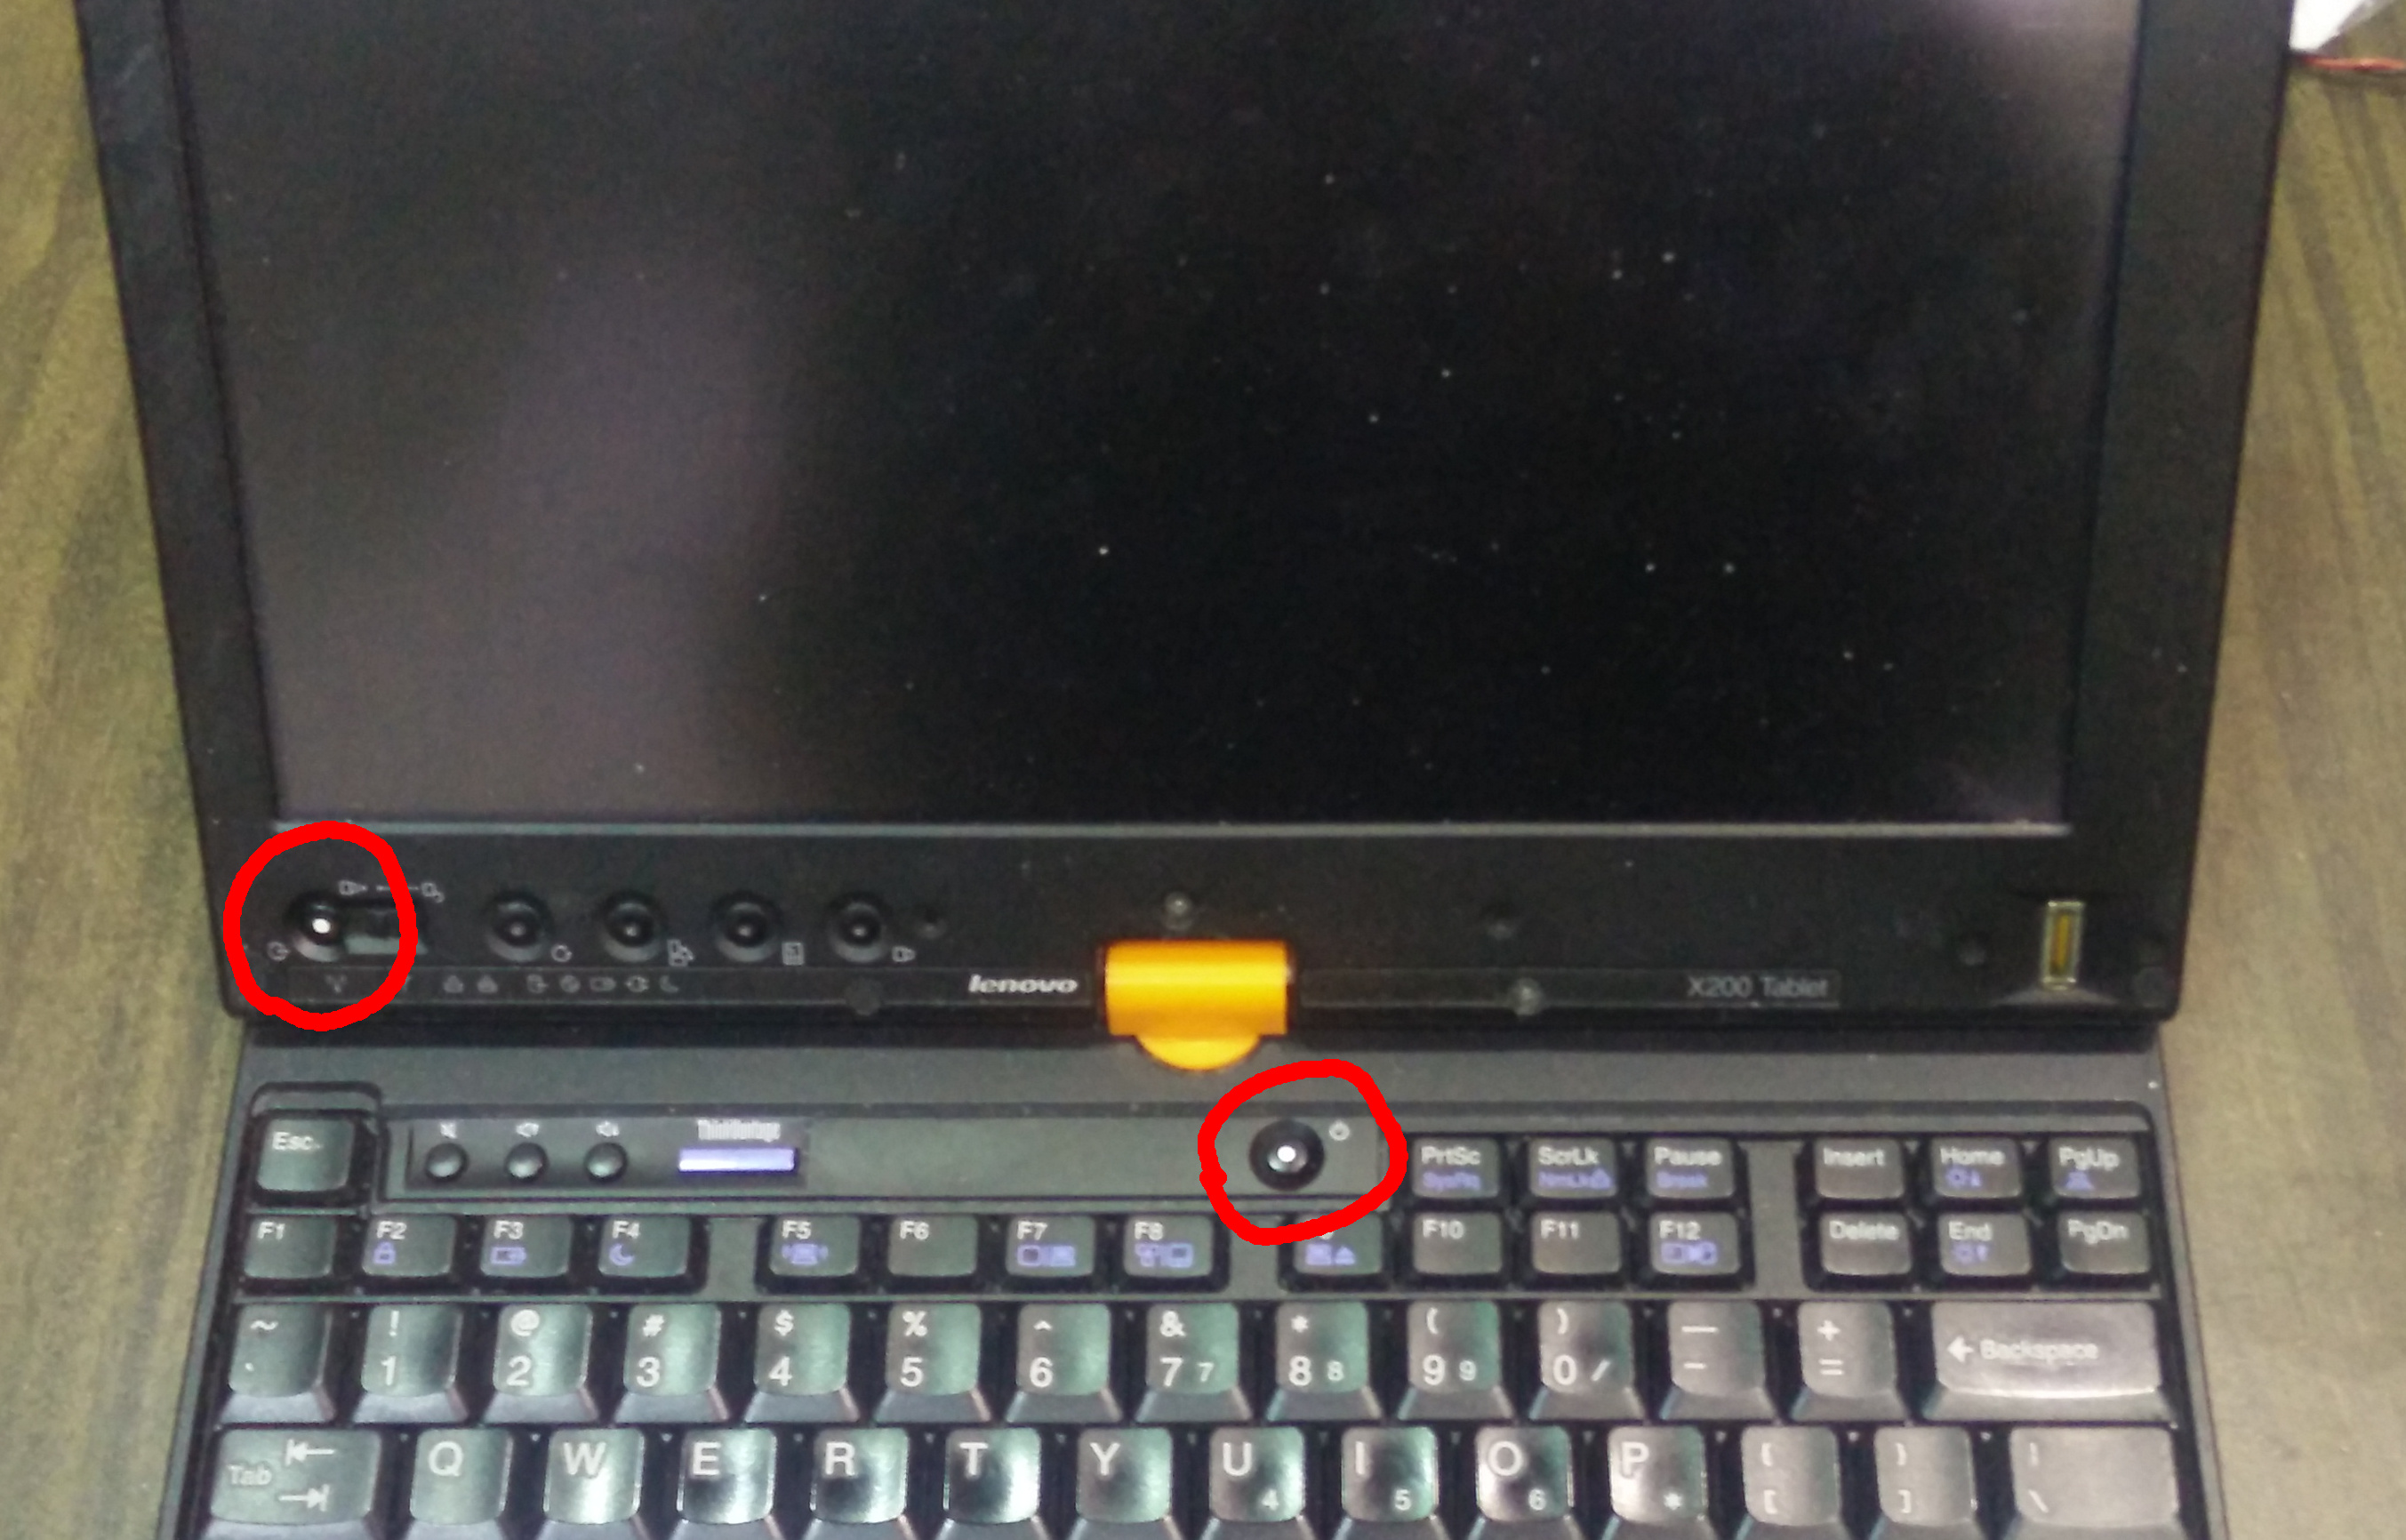
\includegraphics[width=0.5\textwidth]{powerbutton.jpg}
		\caption{Location of the power buttons}
	\end{figure}

	\item Remove the battery and charging connector from the laptop.
	\begin{figure}[H]
		\centering
		\begin{minipage}{0.45\textwidth}
			\centering
			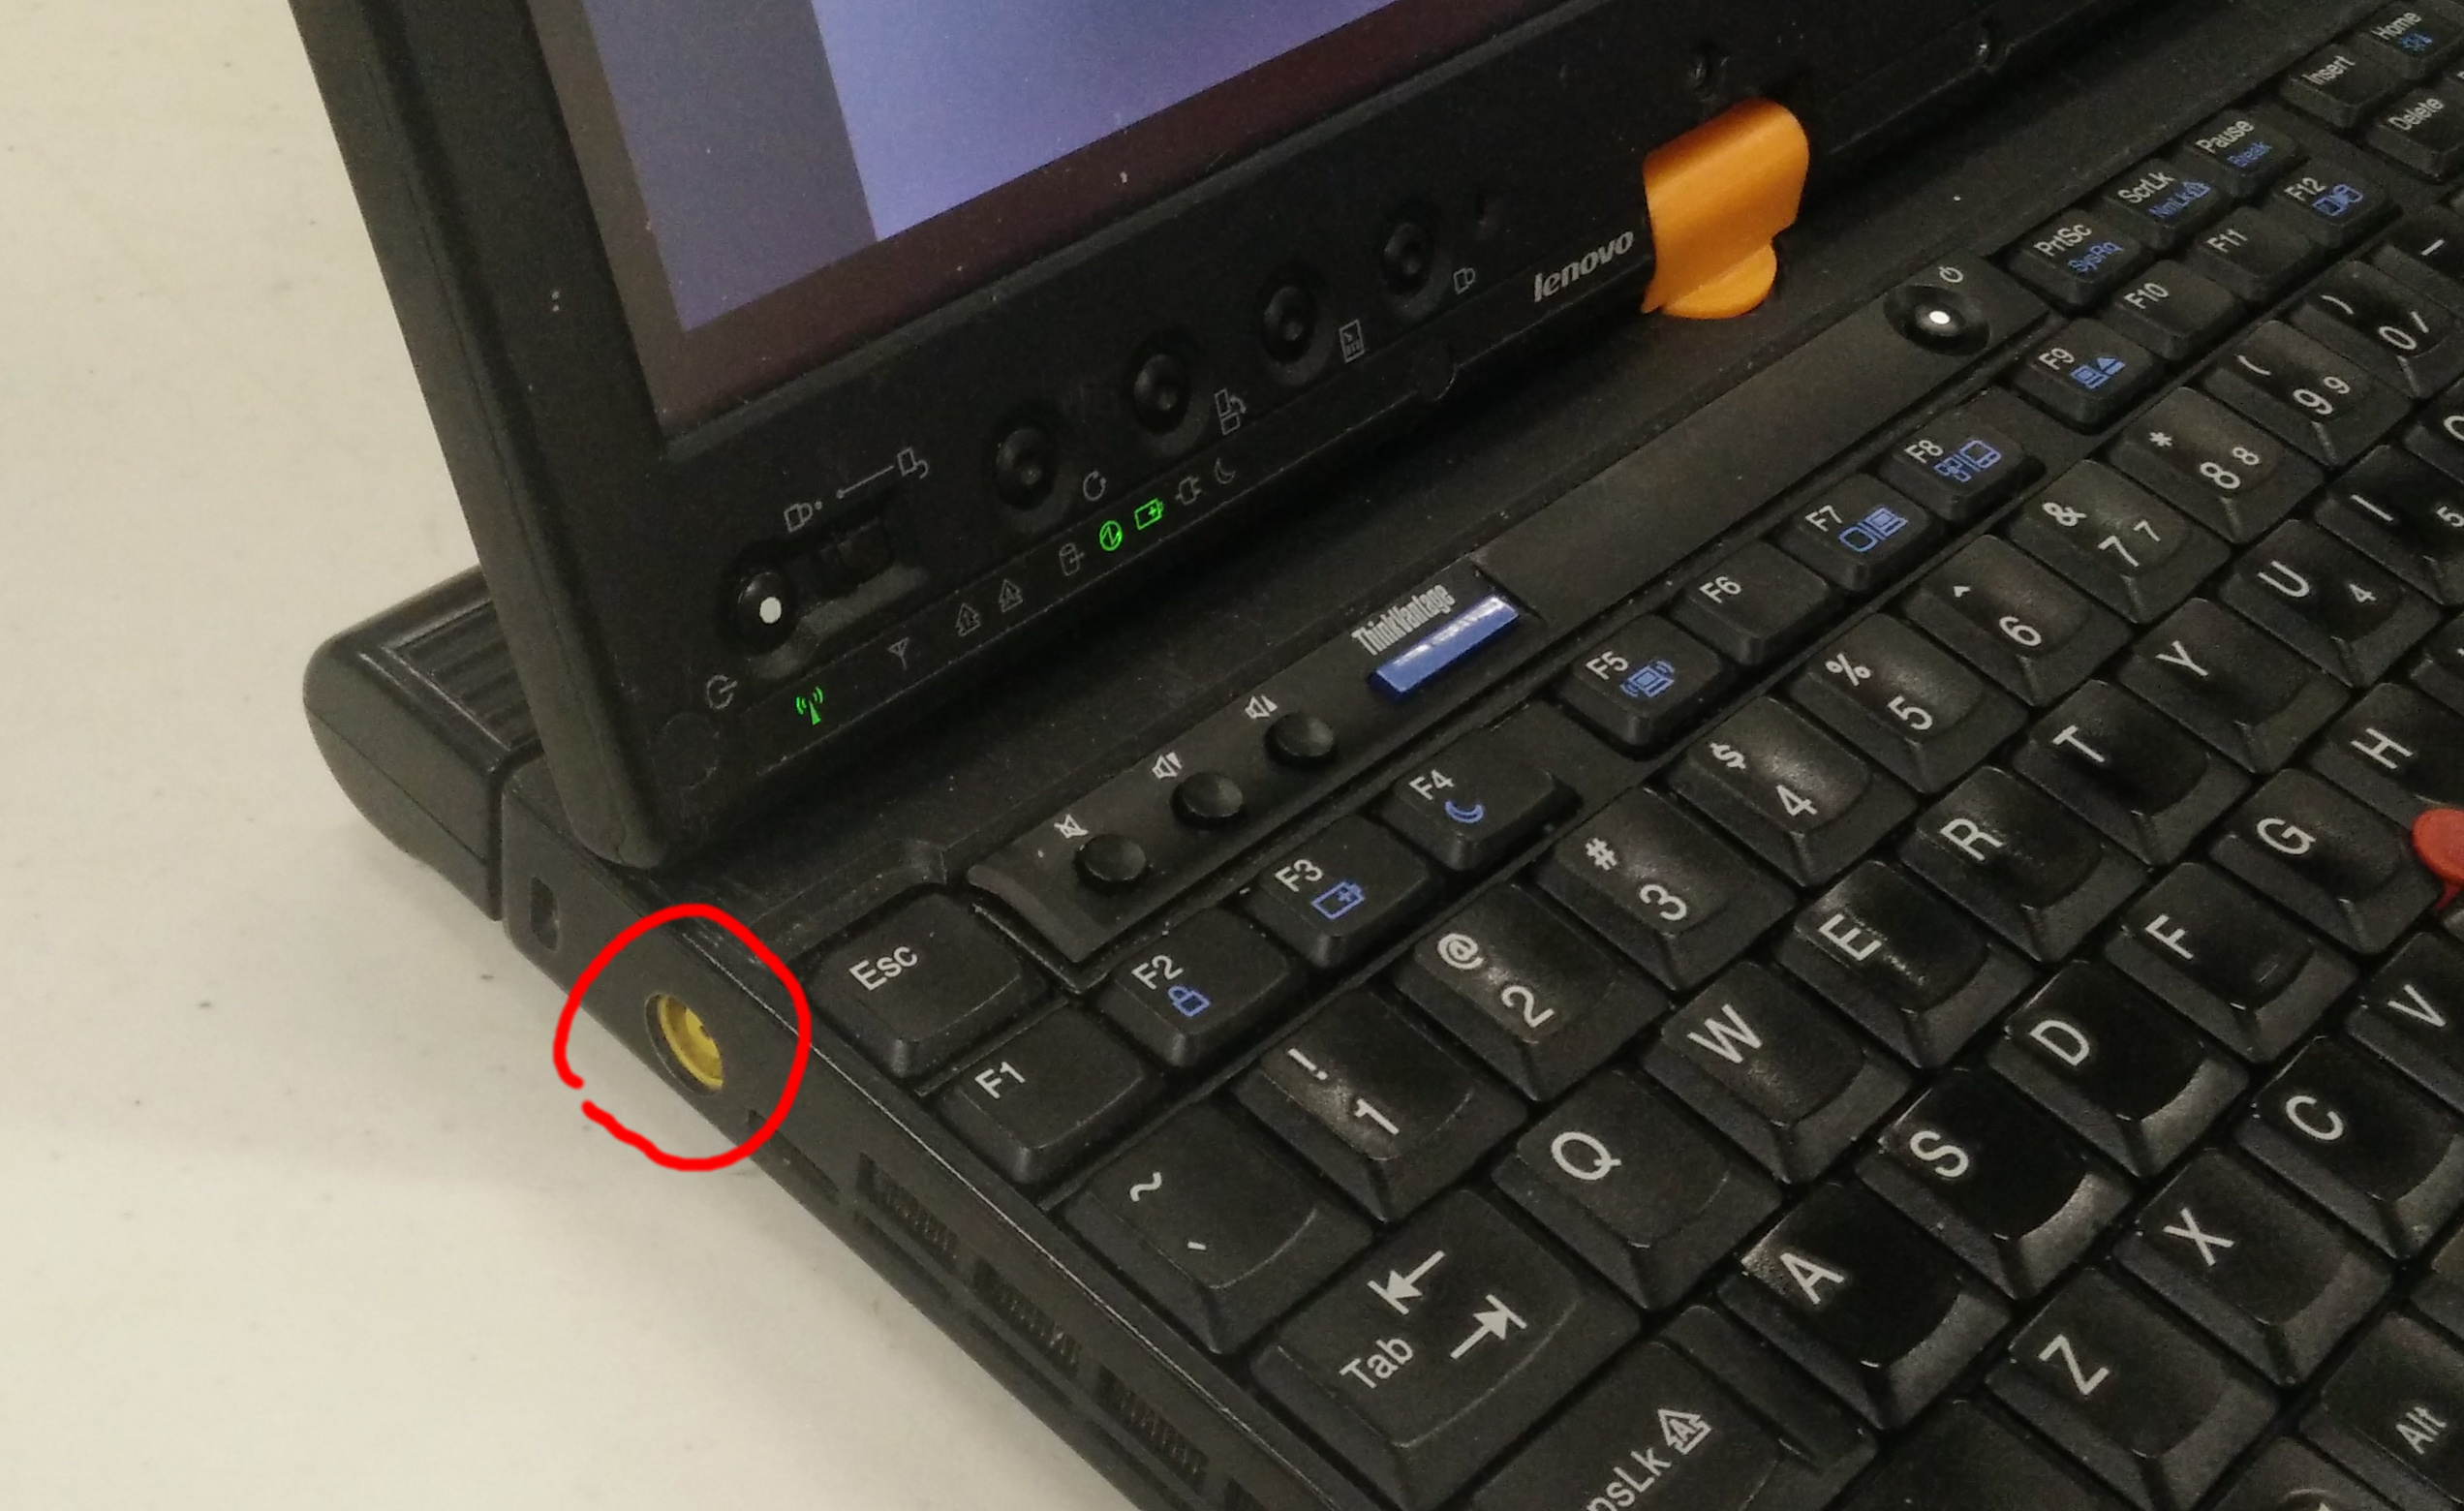
\includegraphics[width=0.9\textwidth]{charger.jpg}
			\caption{Location of the charging port}
		\end{minipage} \hfill
		\begin{minipage}{0.45\textwidth}
			\centering
			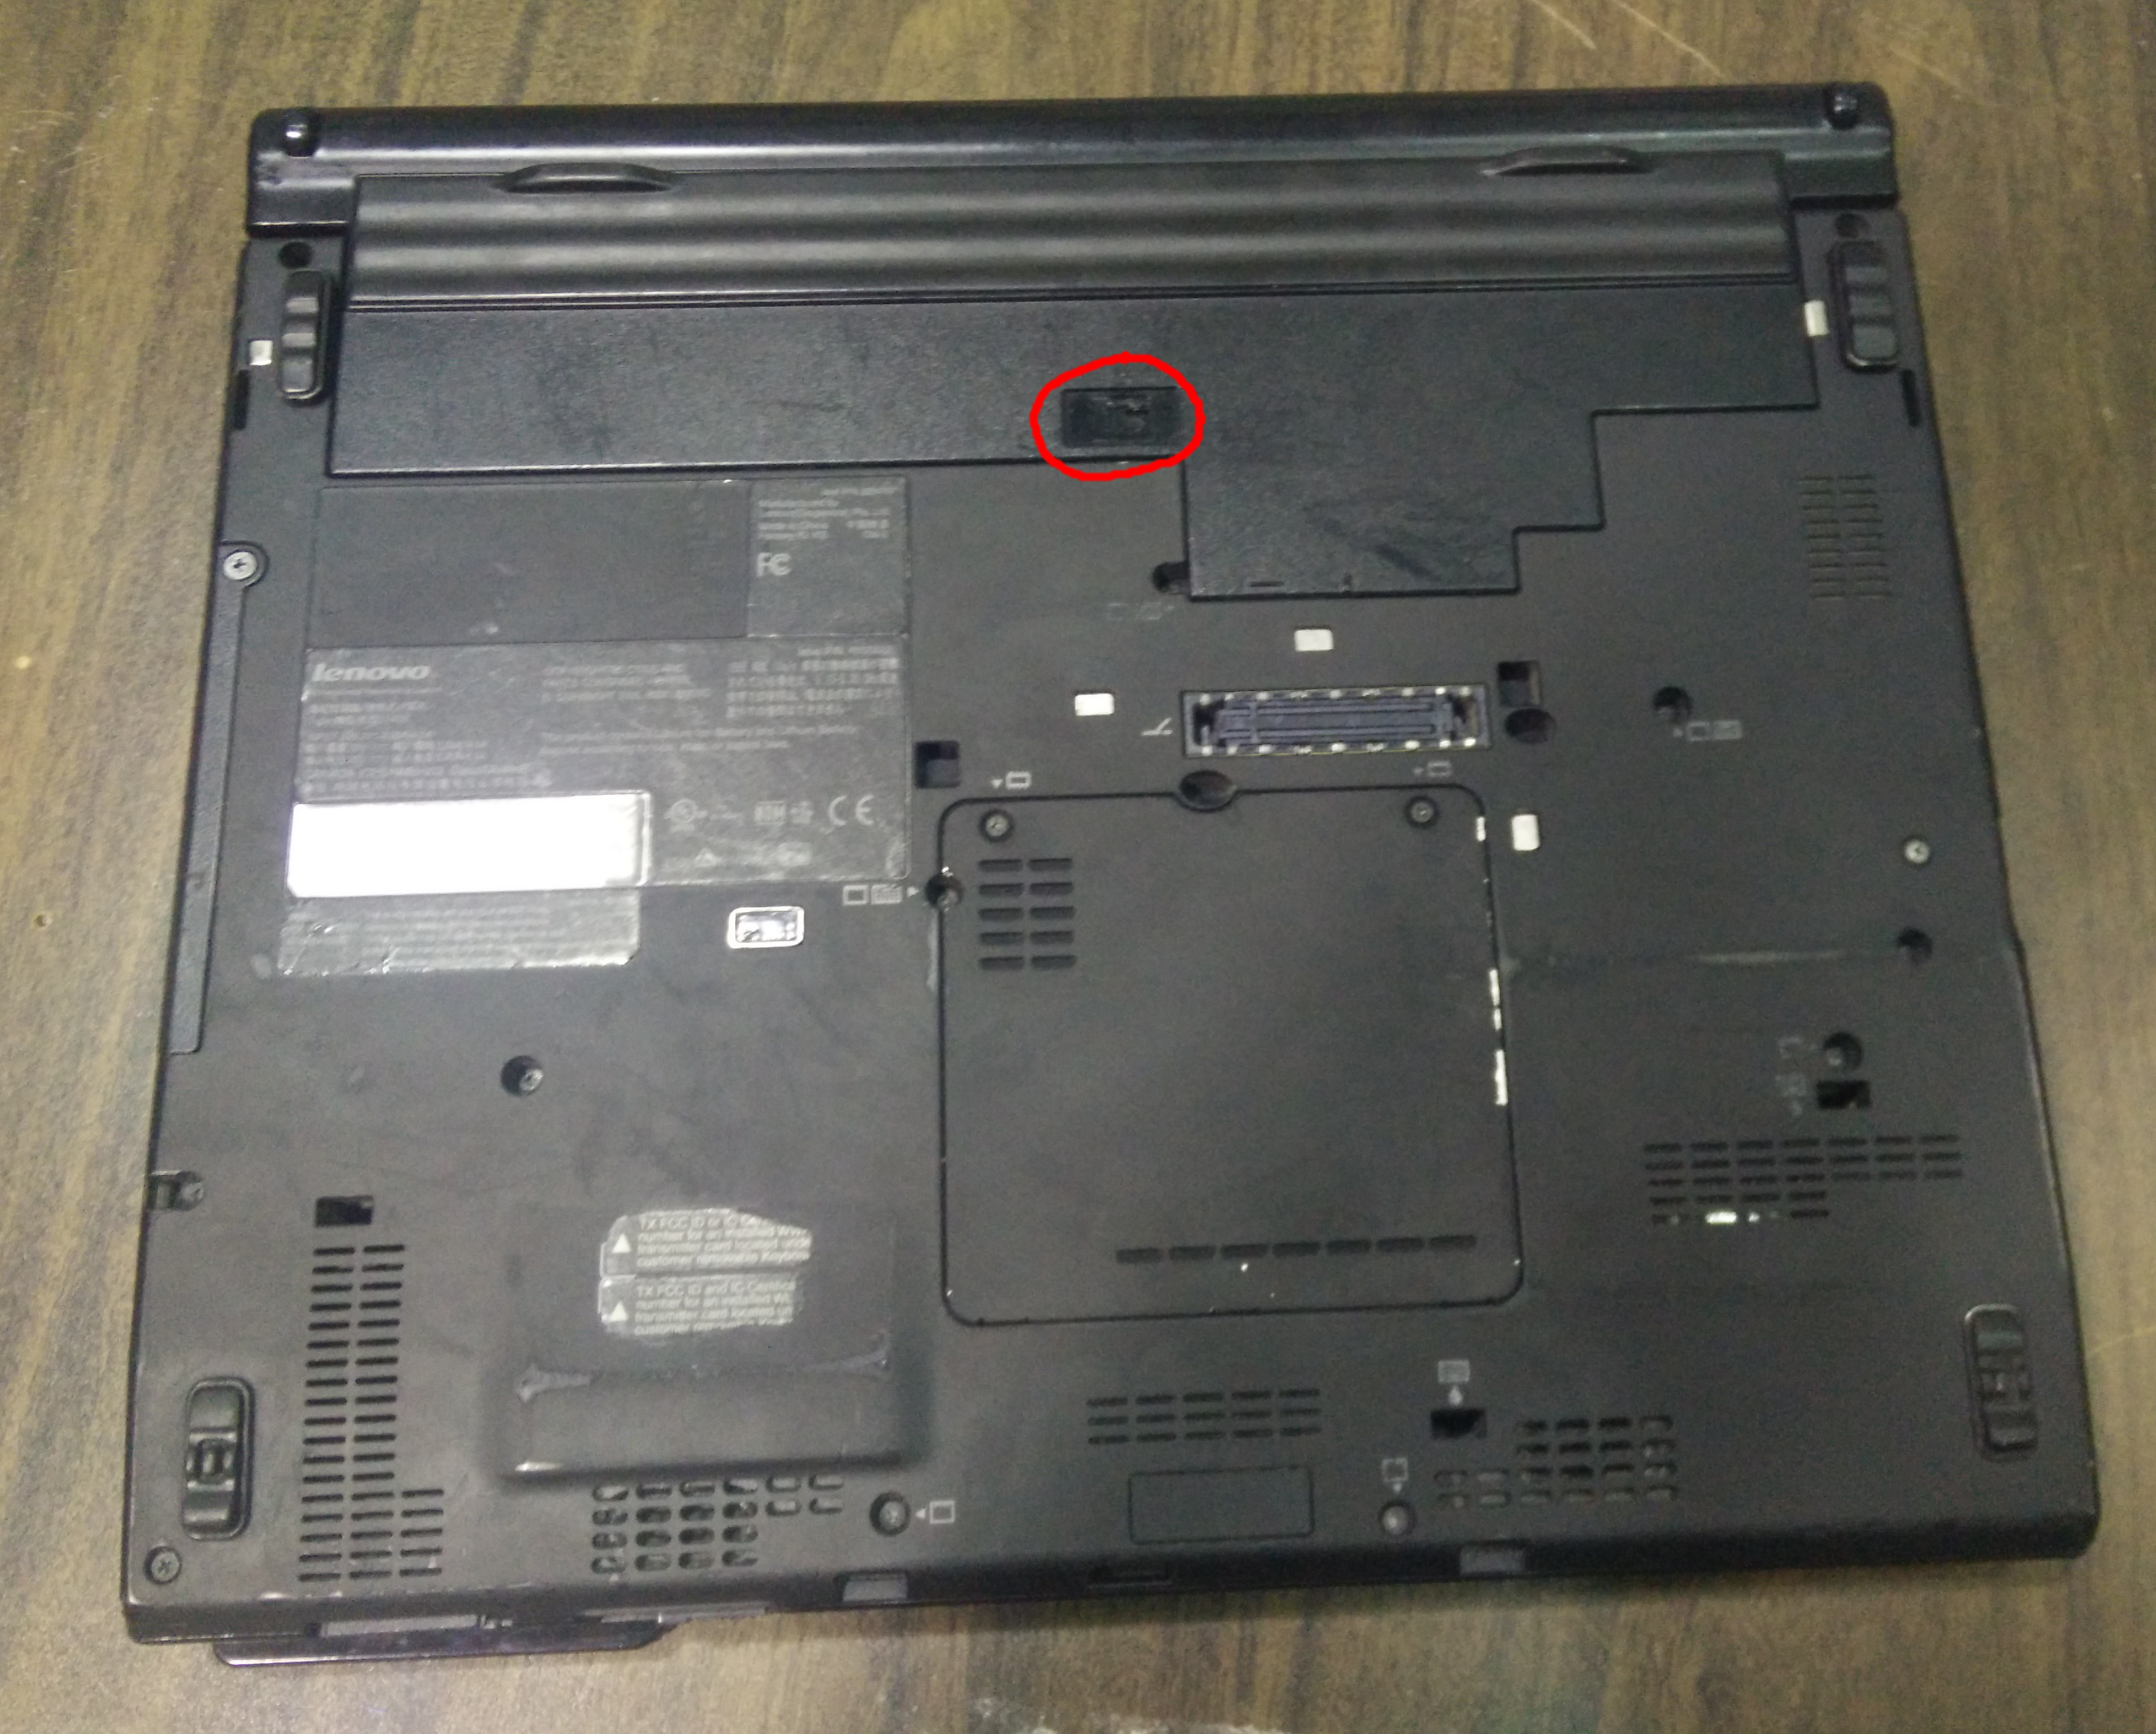
\includegraphics[width=0.9\textwidth]{battery.jpg}
			\caption{Location of the battery removal latch}
		\end{minipage}
	\end{figure}

	\item Press and hold the power button for 10 more seconds to fully discharge any electrcity still stored inside the computer.
	\alertwarningbox{CAUTION: RISK OF DAMAGE}{
		Failure to make sure that there is no residual charge left in the computer may result in damage to the motherboard or other components.
	}

	\clearpage
	\item Remove the four black screws with the keyboard symbol from the bottom of the laptop
	\begin{figure}[H]
		\centering
		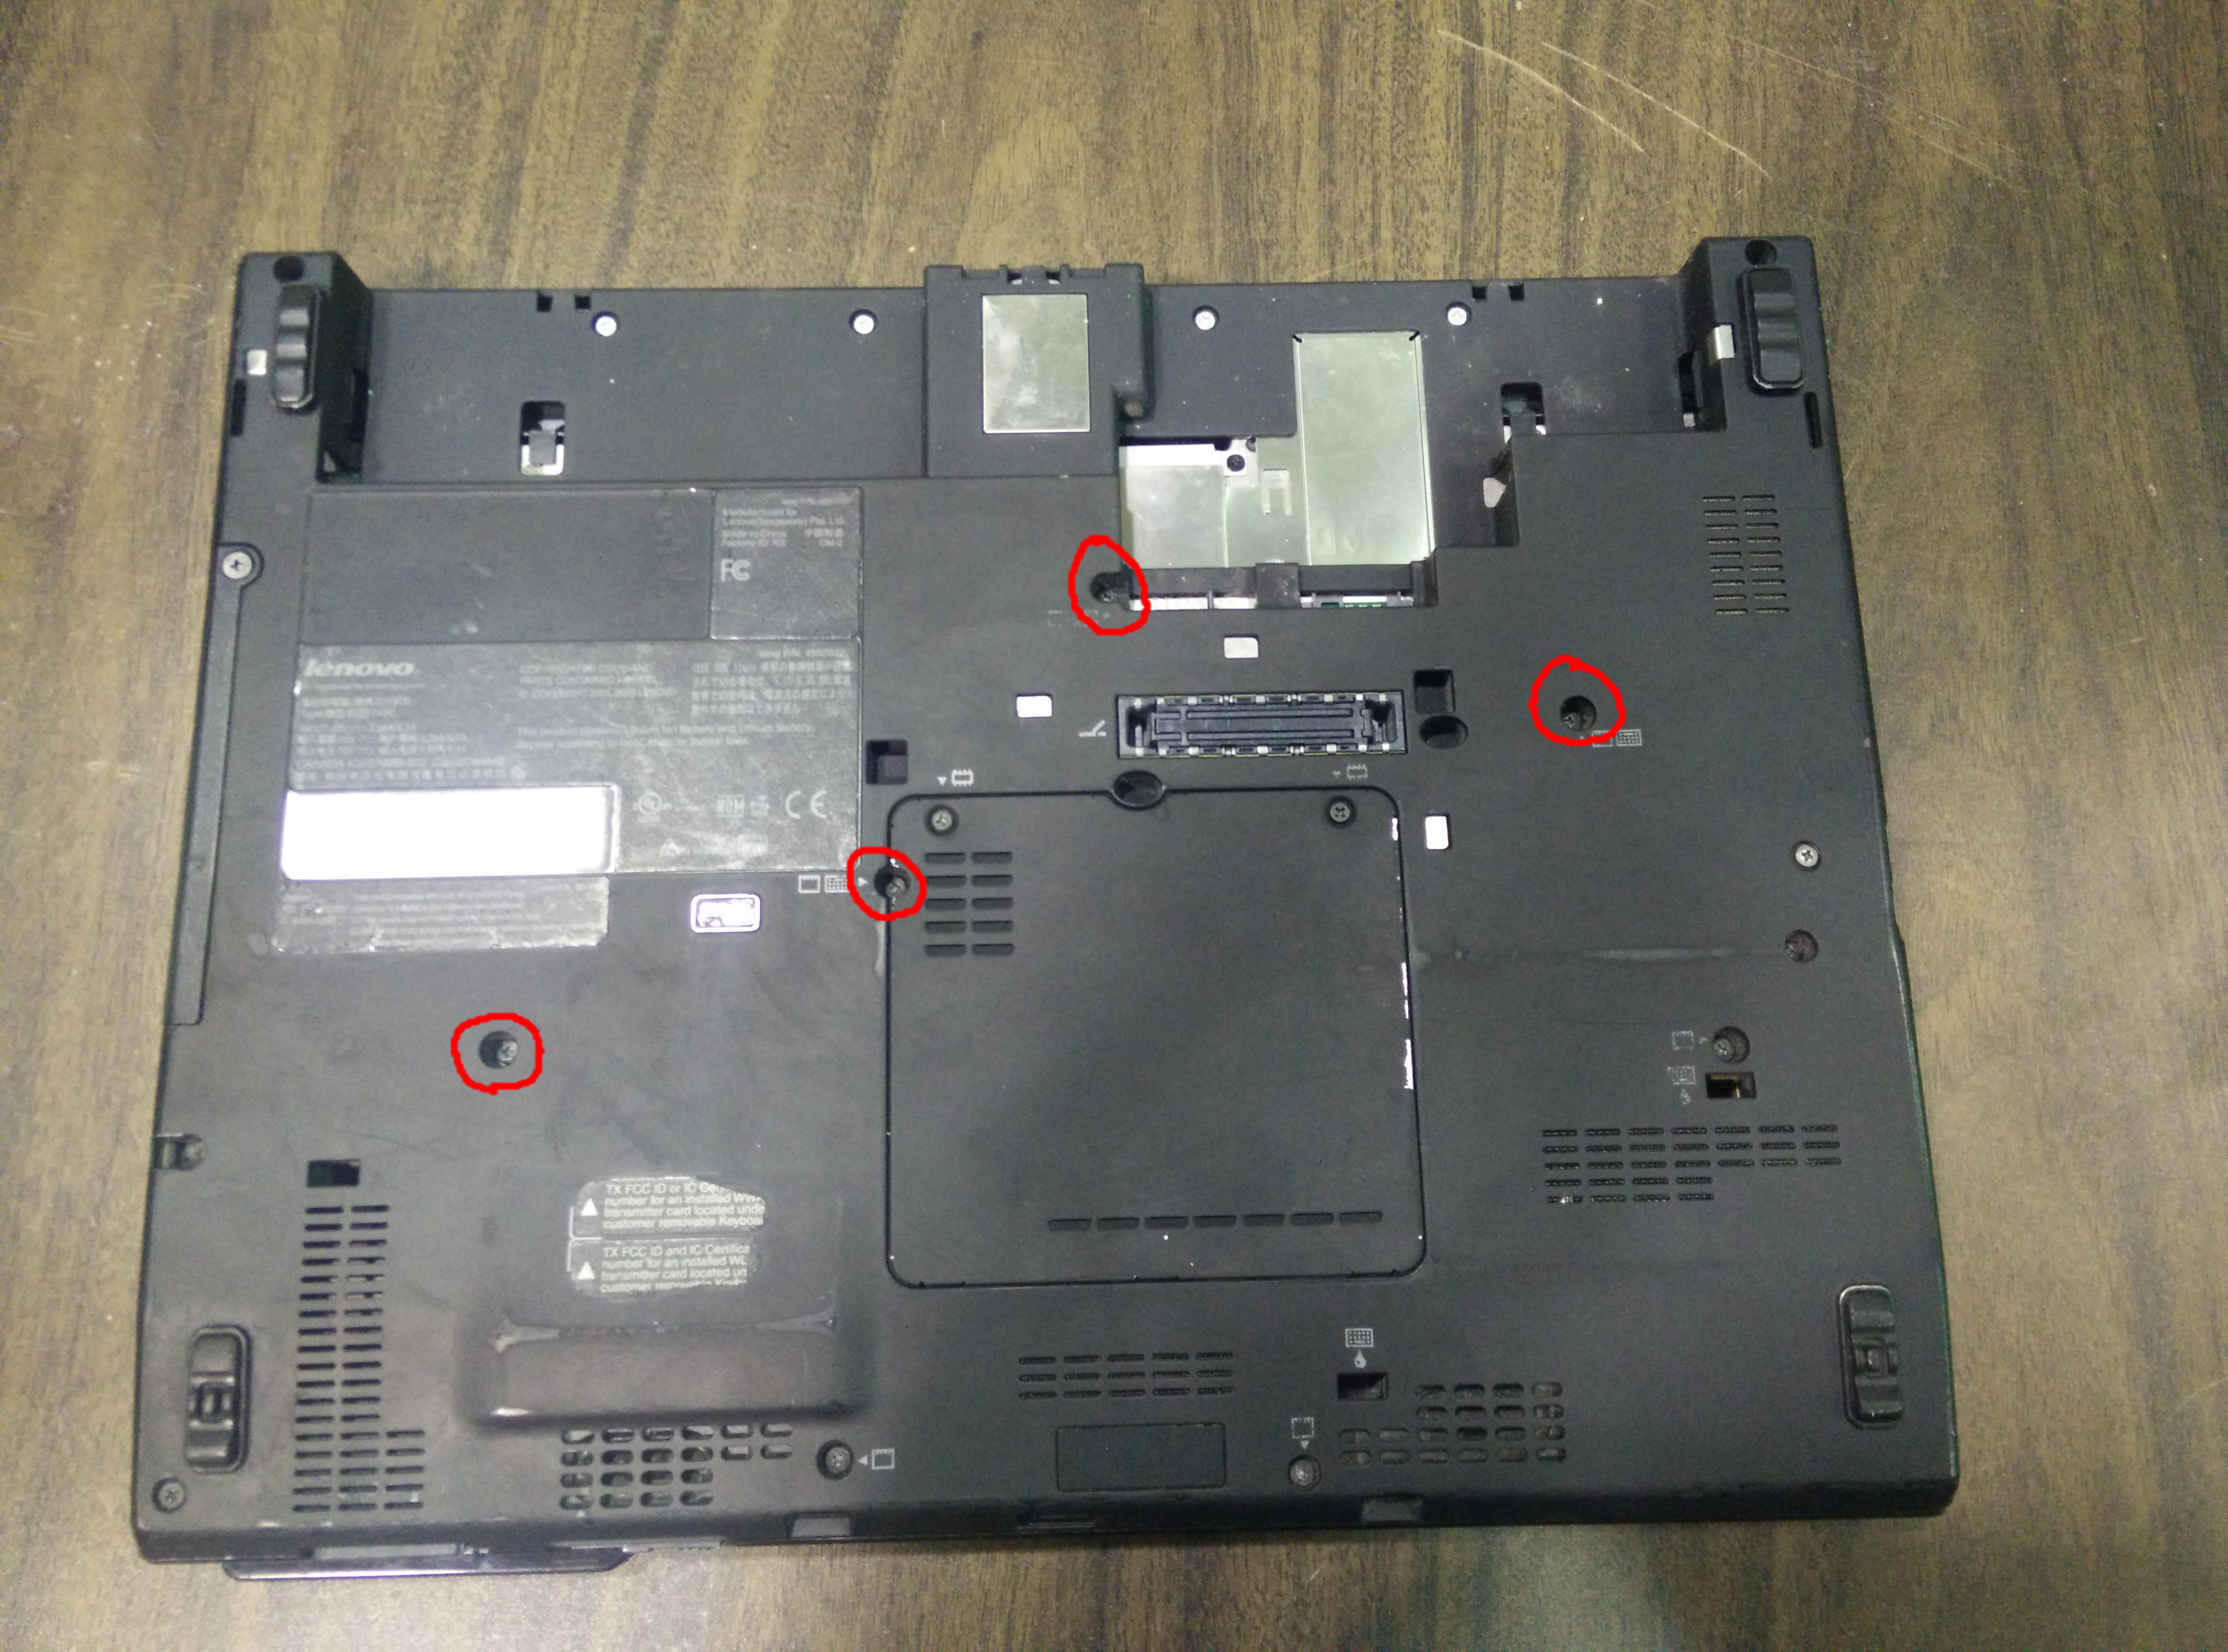
\includegraphics[width=0.7\textwidth]{keyboardscrews.jpg}
		\caption{Location of the four keyboard screws}
		\label{fig:screws}
	\end{figure}

	\alertinfobox{INFO}{
		The screws are very small and easy to lose, keep them in a safe place as soon as you take them out.
	}

	\item Put pressure on the keyboard and slide it towards the screen until the retaining tabs near the bottom of the keyboard are clear of the palm rest.
	\begin{figure}[H]
		\centering
		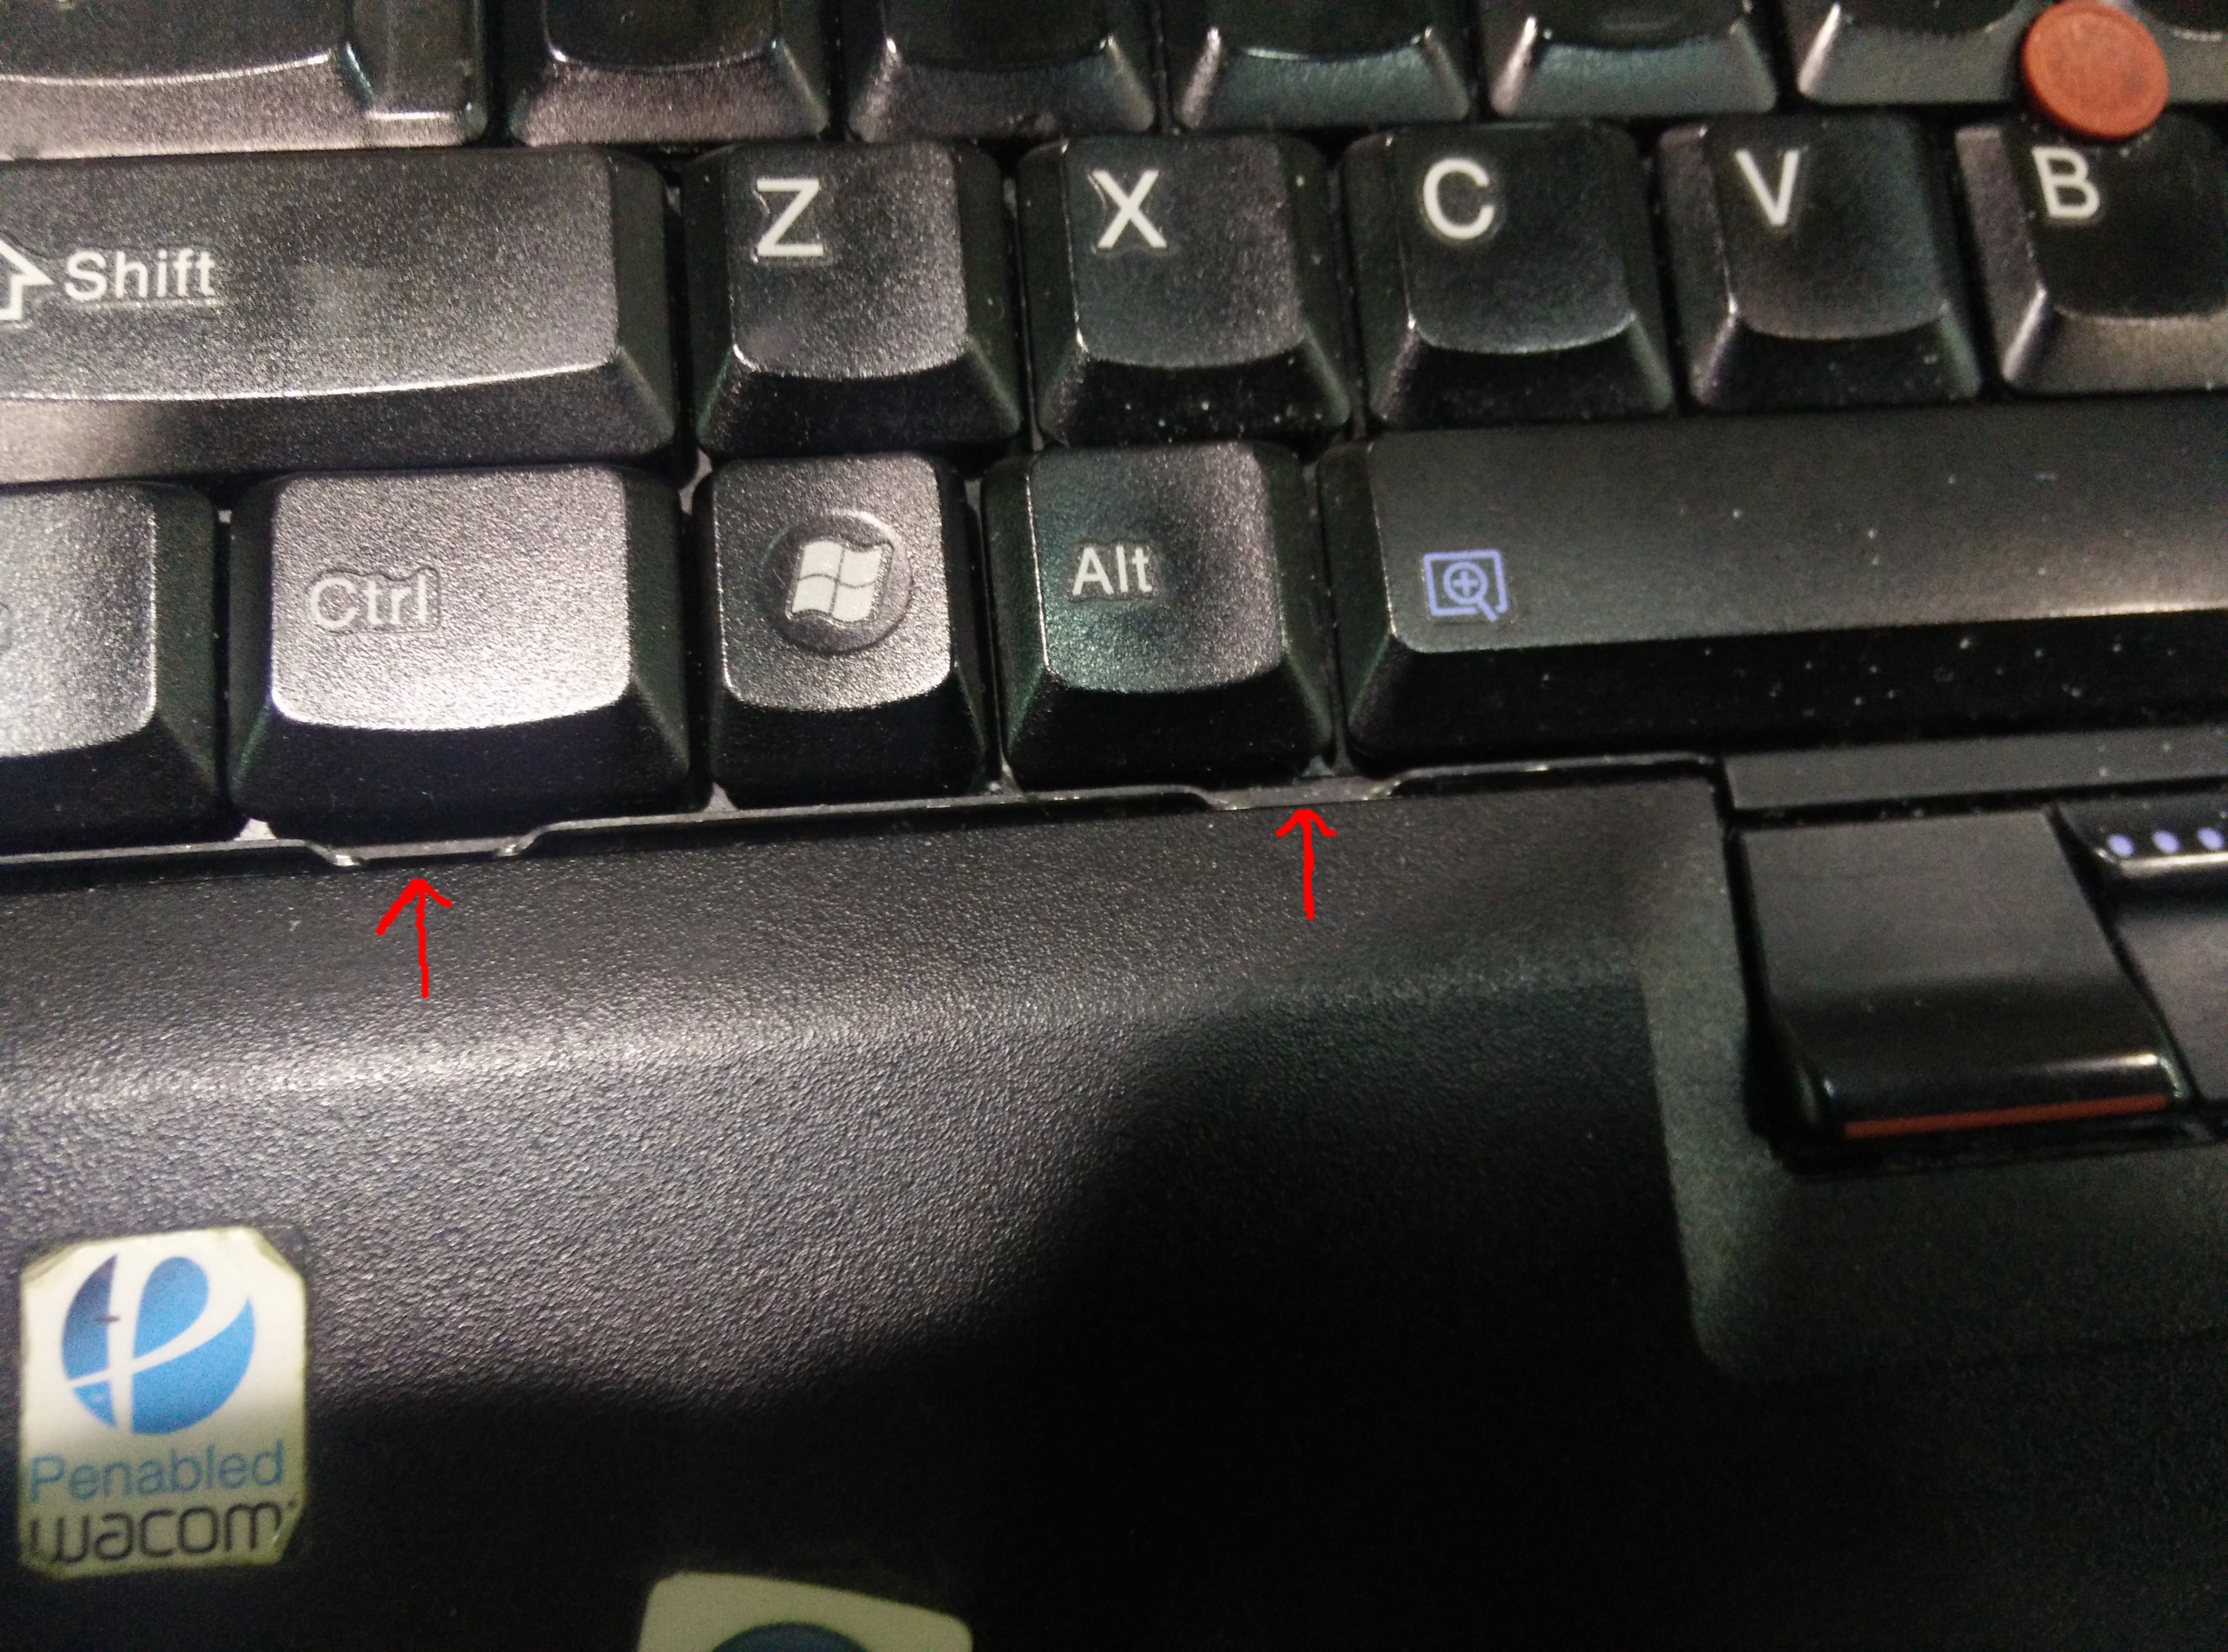
\includegraphics[width=0.6\textwidth]{keyboardslide.jpg}
		\caption{Retaining tabs on the keyboard}
	\end{figure}

	\item Once the retaining tabs are clear, the board should begin to lift out.
	Carefully raise the keyboard out of the housing and lay it  on the screen.
	\begin{figure}[H]
		\centering
		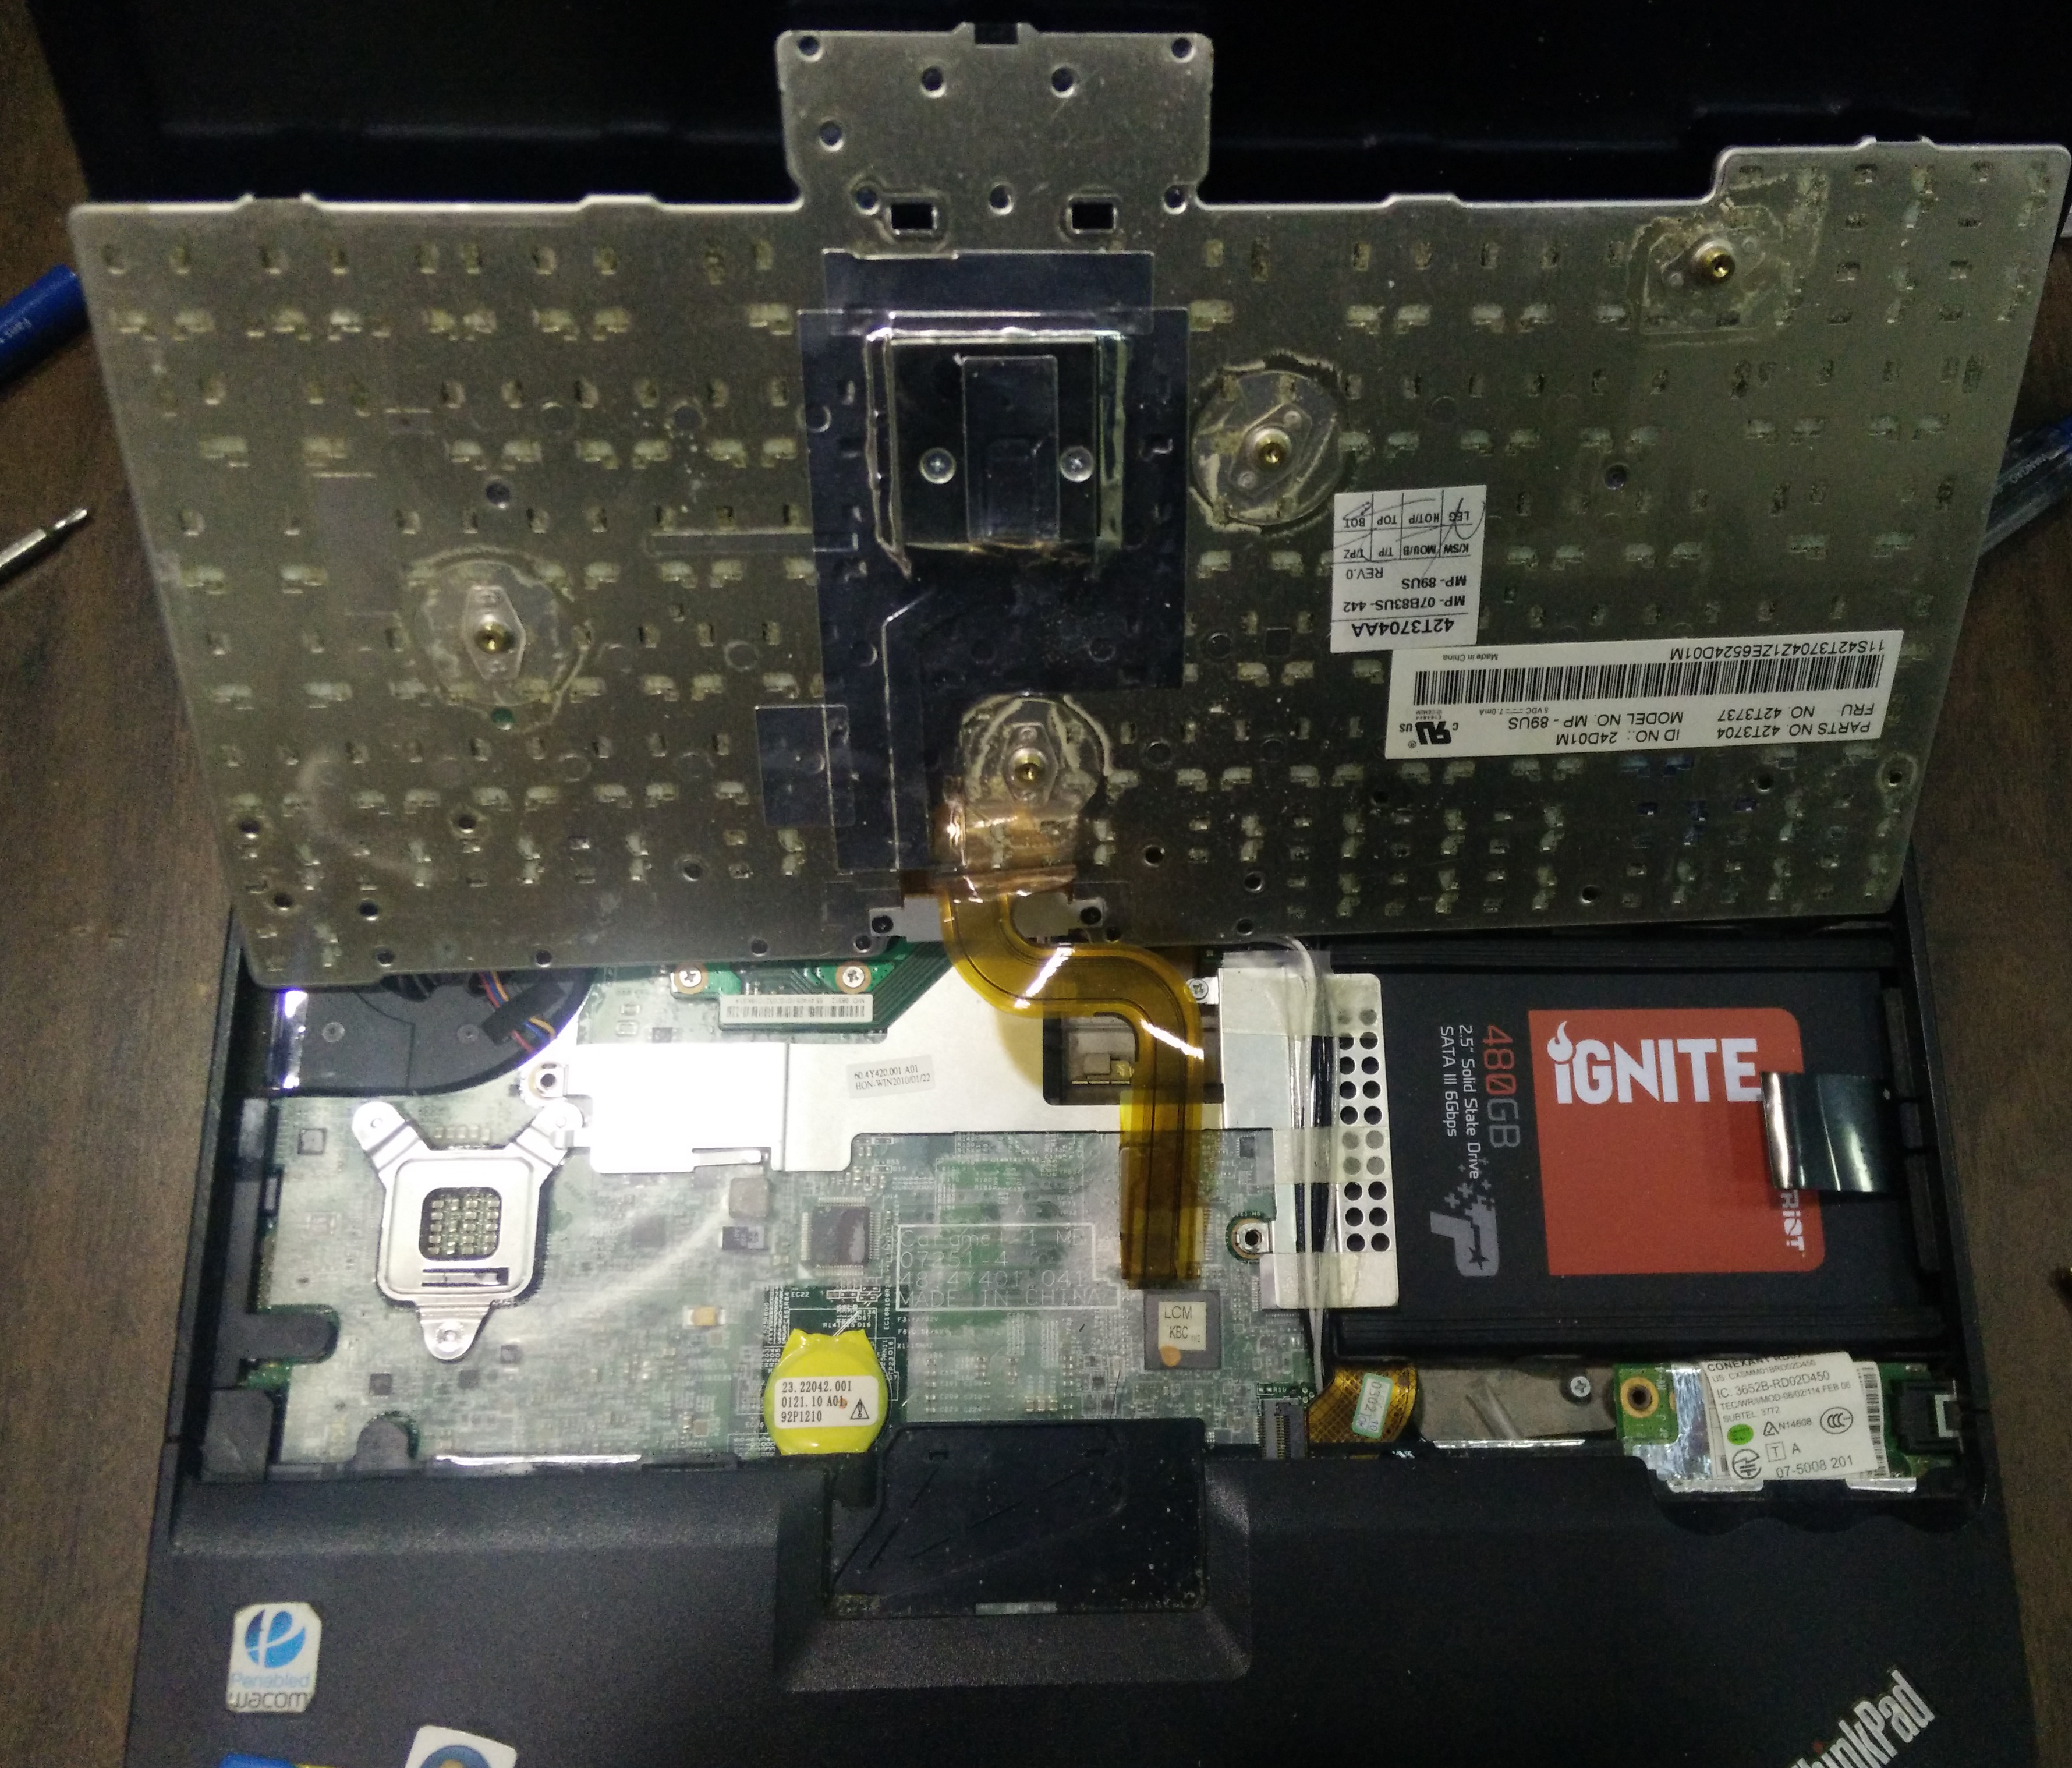
\includegraphics[width=0.5\textwidth]{keyboardonscreen.jpg}
		\caption{Keyboard removed from the housing}
	\end{figure}

	\alertwarningbox{CAUTION: RISK OF DAMAGE}{
		The keyboard is connected to the laptop motherboard by a fragile ribbon cable, do not pull the keyboard away from the computer before removing it.
	}

	\item Carefully remove the keyboard connector from the laptop motherboard by pulling upwards on the pulltab.
		The keyboard is now completely free from the computer.
	\begin{figure}[H]
		\centering
		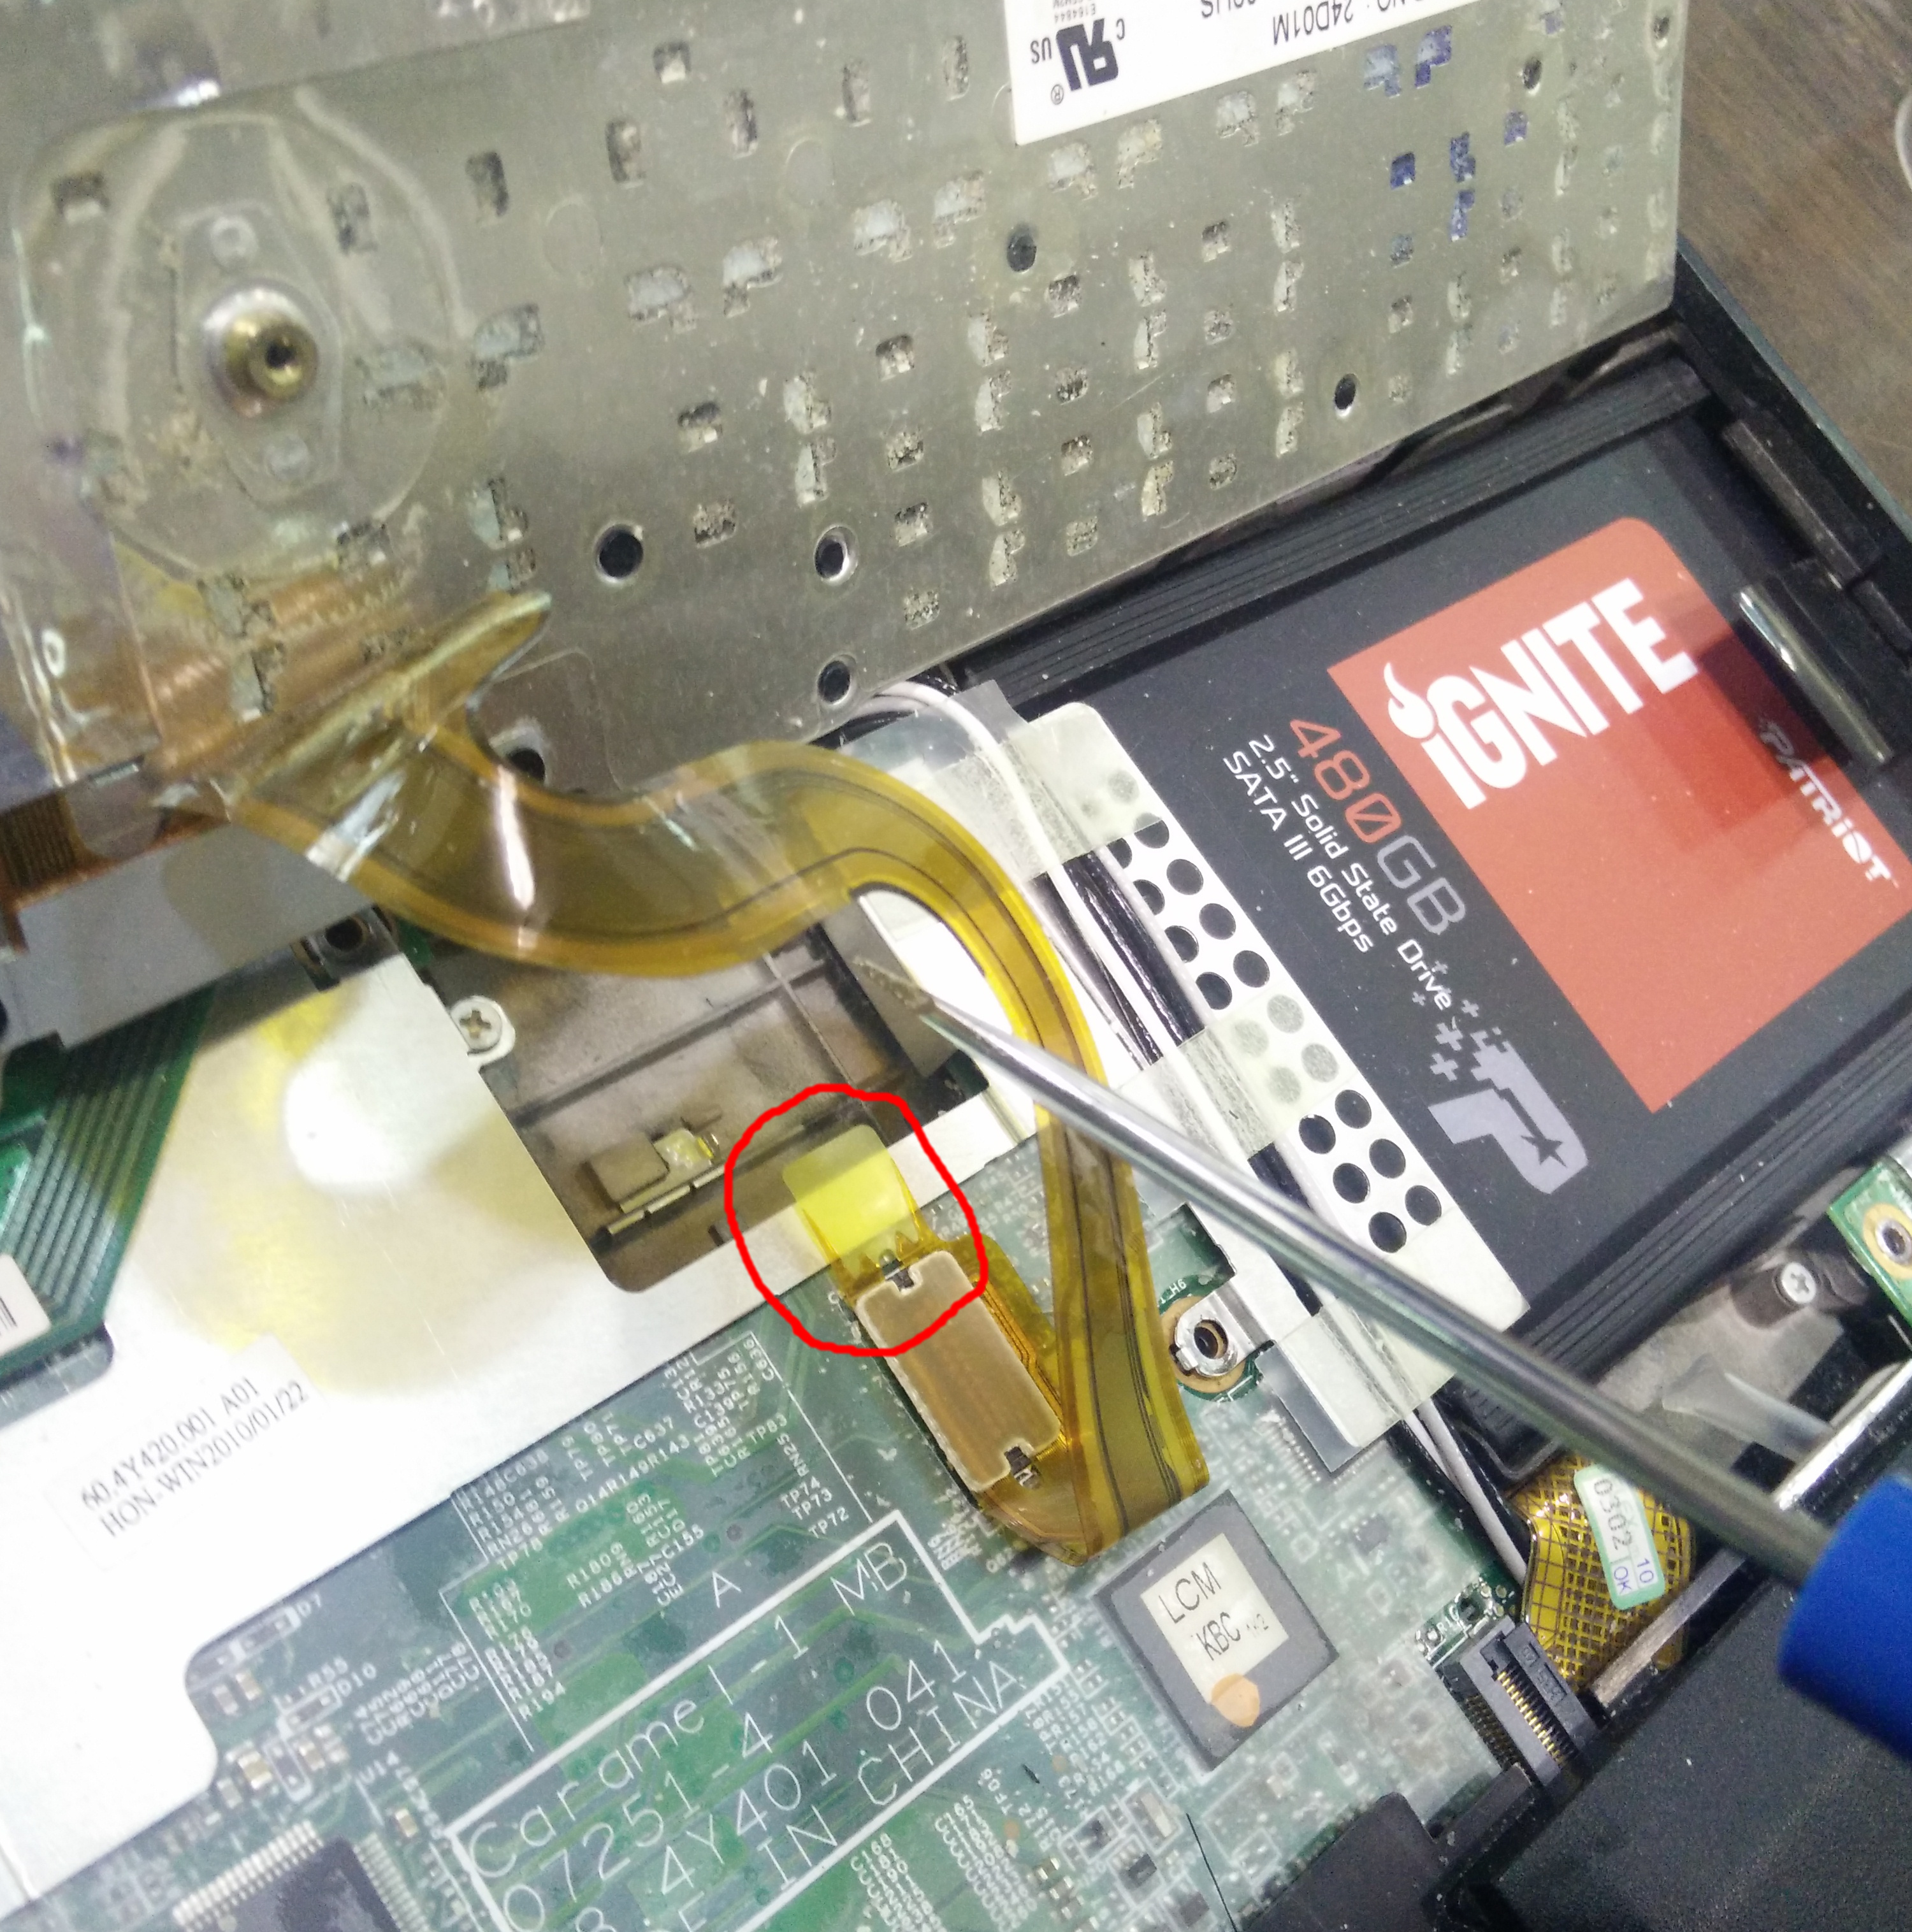
\includegraphics[width=0.5\textwidth]{keyboardconnectortab.jpg}
		\caption{The connector tab of the keyboard}
	\end{figure}

\end{enumerate}

\clearpage

\section*{Cleaning the keyboard}
\begin{enumerate}
	\item Spray compressed air into the crevices of the keyboard in order to clear out the dust stuck in it.

	\begin{figure}[H]
		\centering
		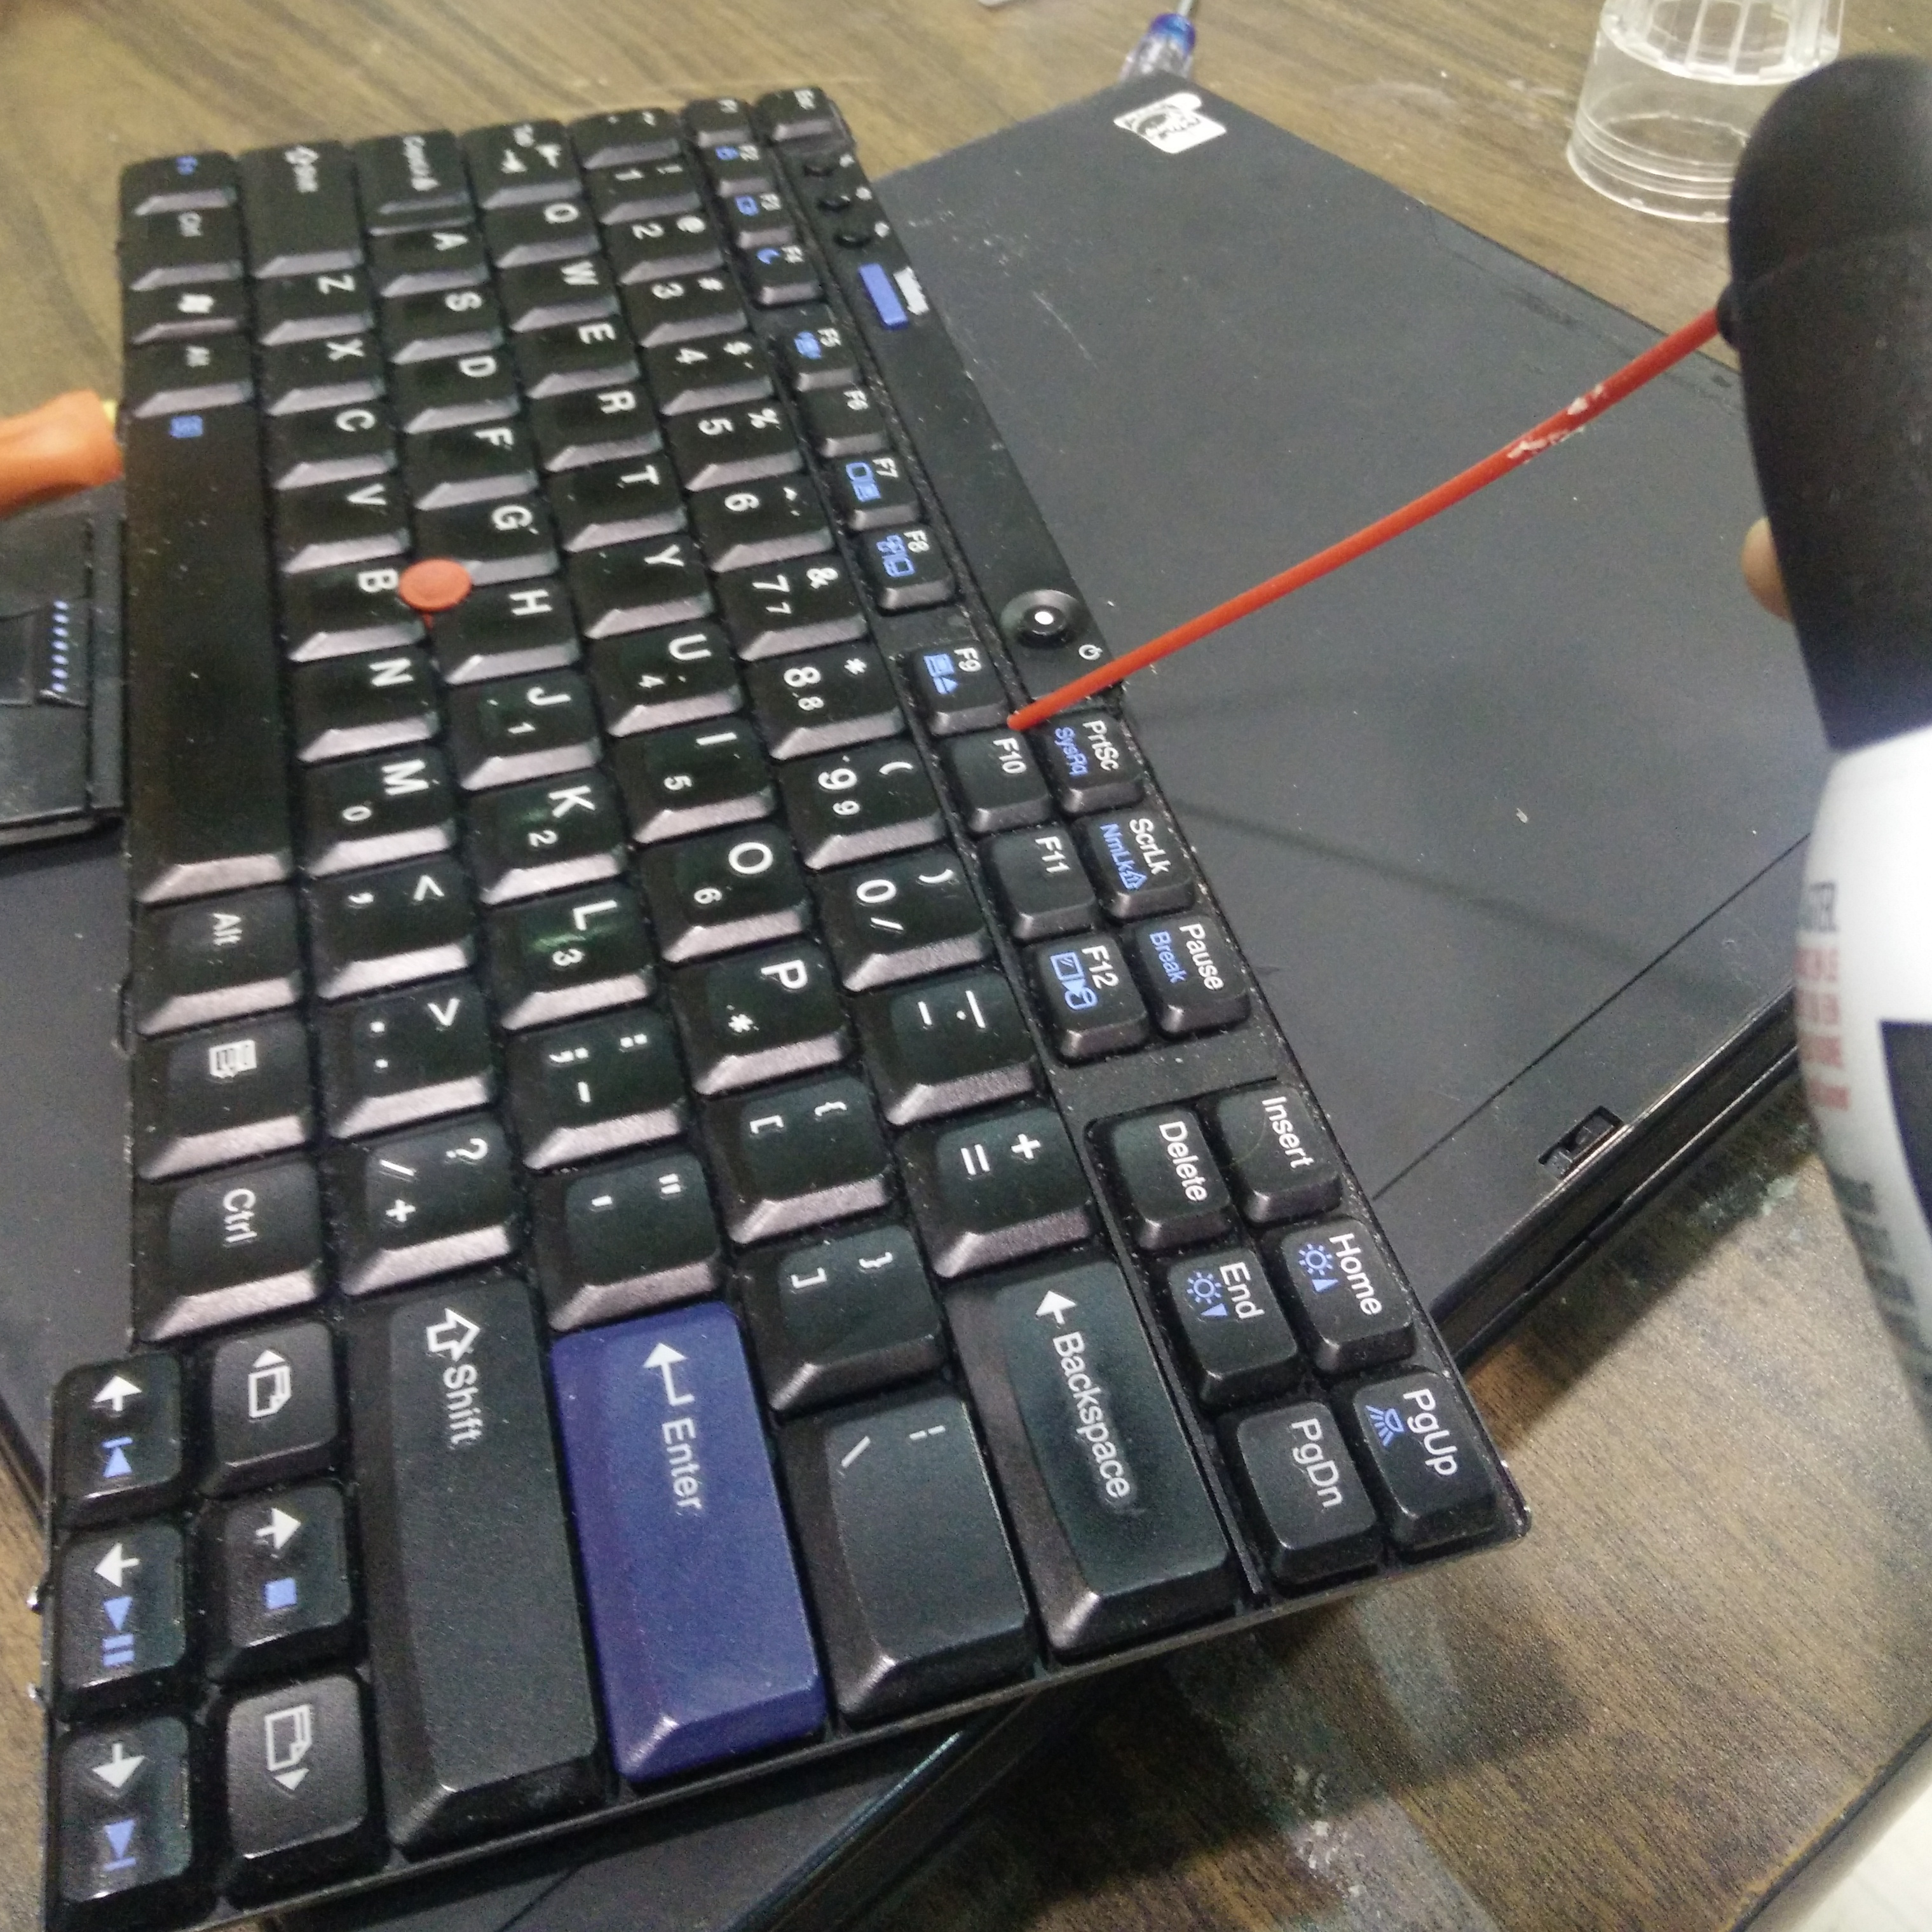
\includegraphics[width=0.5\textwidth]{aircankeyboard.jpg}
		\caption{Using compressed air to blow out dust particles on the keyboard}
	\end{figure}

	\alertinfobox{INFO}{
		It may be hard to get everything out, so you may want to also remove the individual keycaps.
		To do so, gently pry up the underside of the key until it pops off.
	}

	\item Once all of the dust has been removed from the keyboard, pour some isopropyl alcohol onto a cloth and wipe down the keyboard
%	\begin{figure}[H]
%		\centering
%		\includegraphics[width=0.5\textwidth]{wipedownkeyboard.jpg}
%		\caption{Wiping down the keyboard with isopropyl alcohol}
%	\end{figure}

\end{enumerate}

\clearpage

\section*{Replacing the keyboard}
\begin{enumerate}
	\item Reconnect the keyboard connector to the motherboard, making sure that the pulltab is oriented towards the screen.
	\begin{figure}[H]
		\centering
		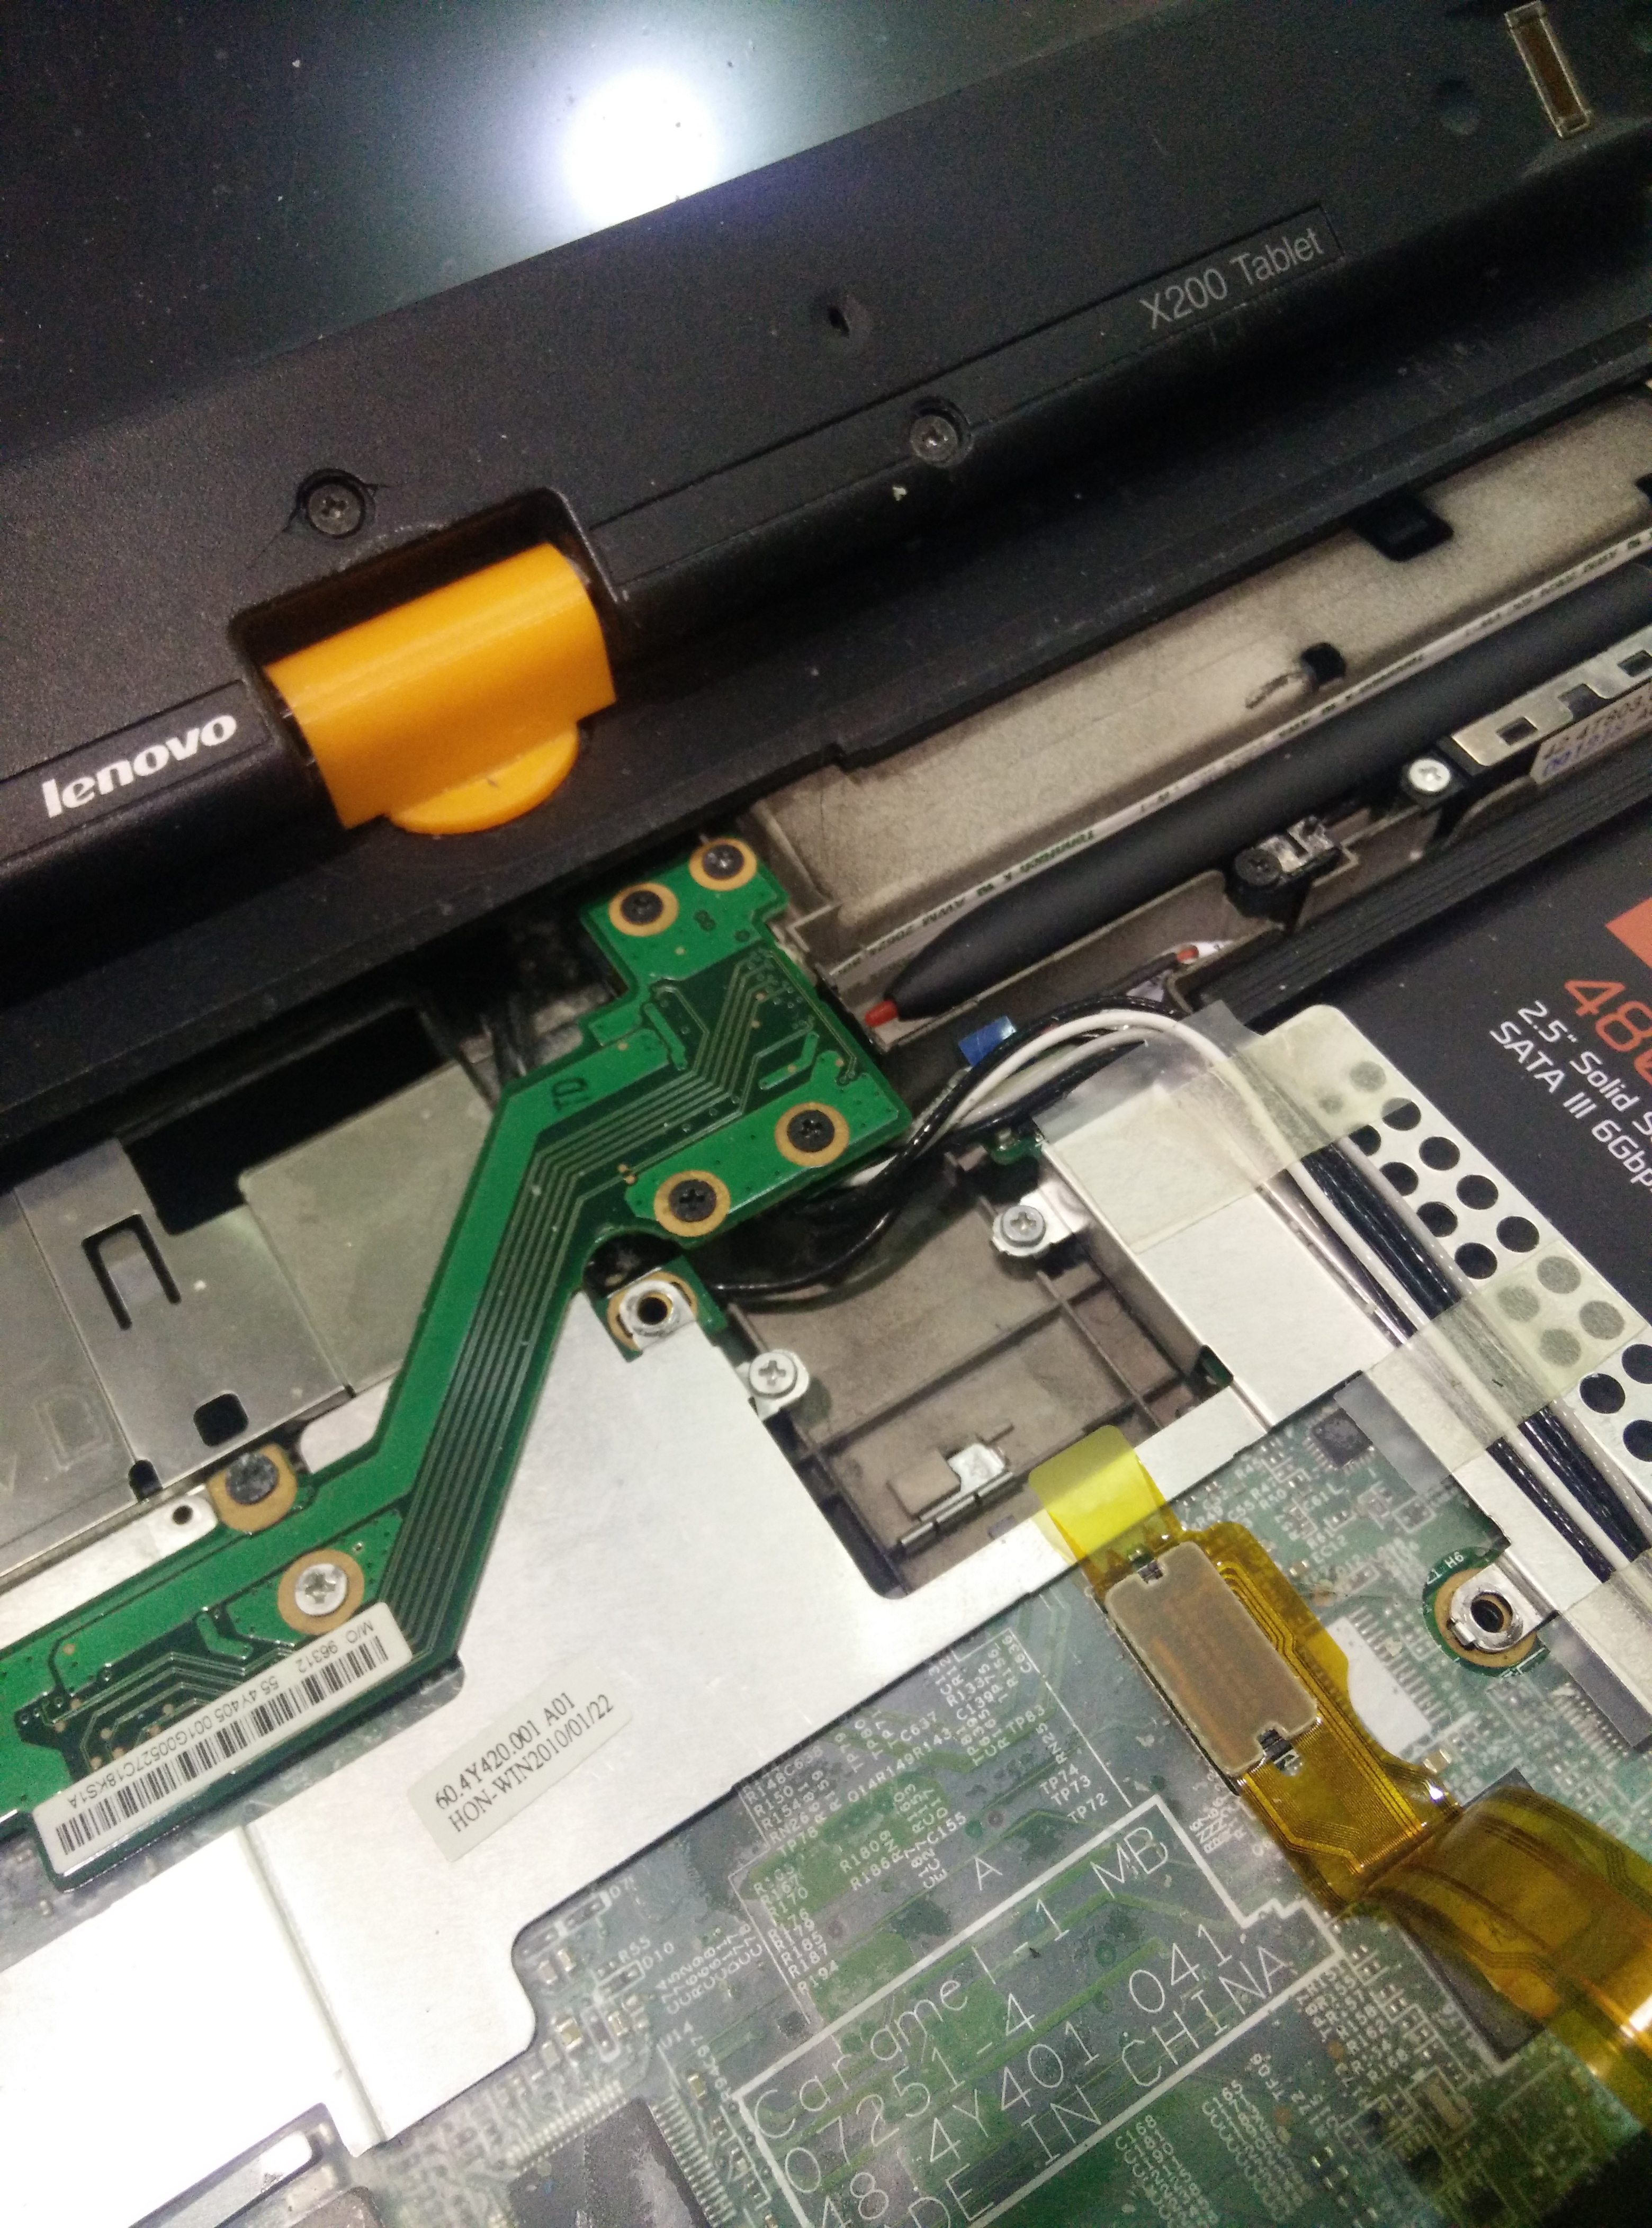
\includegraphics[width=0.5\textwidth]{reconnectkeyboard.jpg}
		\caption{Correct orientation of the keyboard connector}
	\end{figure}

	\alertwarningbox{CAUTION: RISK OF DAMAGE}{
		The keyboard connector should snap in with very little effort, do not put excessive force the connector.
	}

	\clearpage
	\item Begin by inserting the front of the keyboard into the housing at an angle as shown in Figure \ref{fig:angleinsert}.
	\begin{figure}[H]
		\centering
		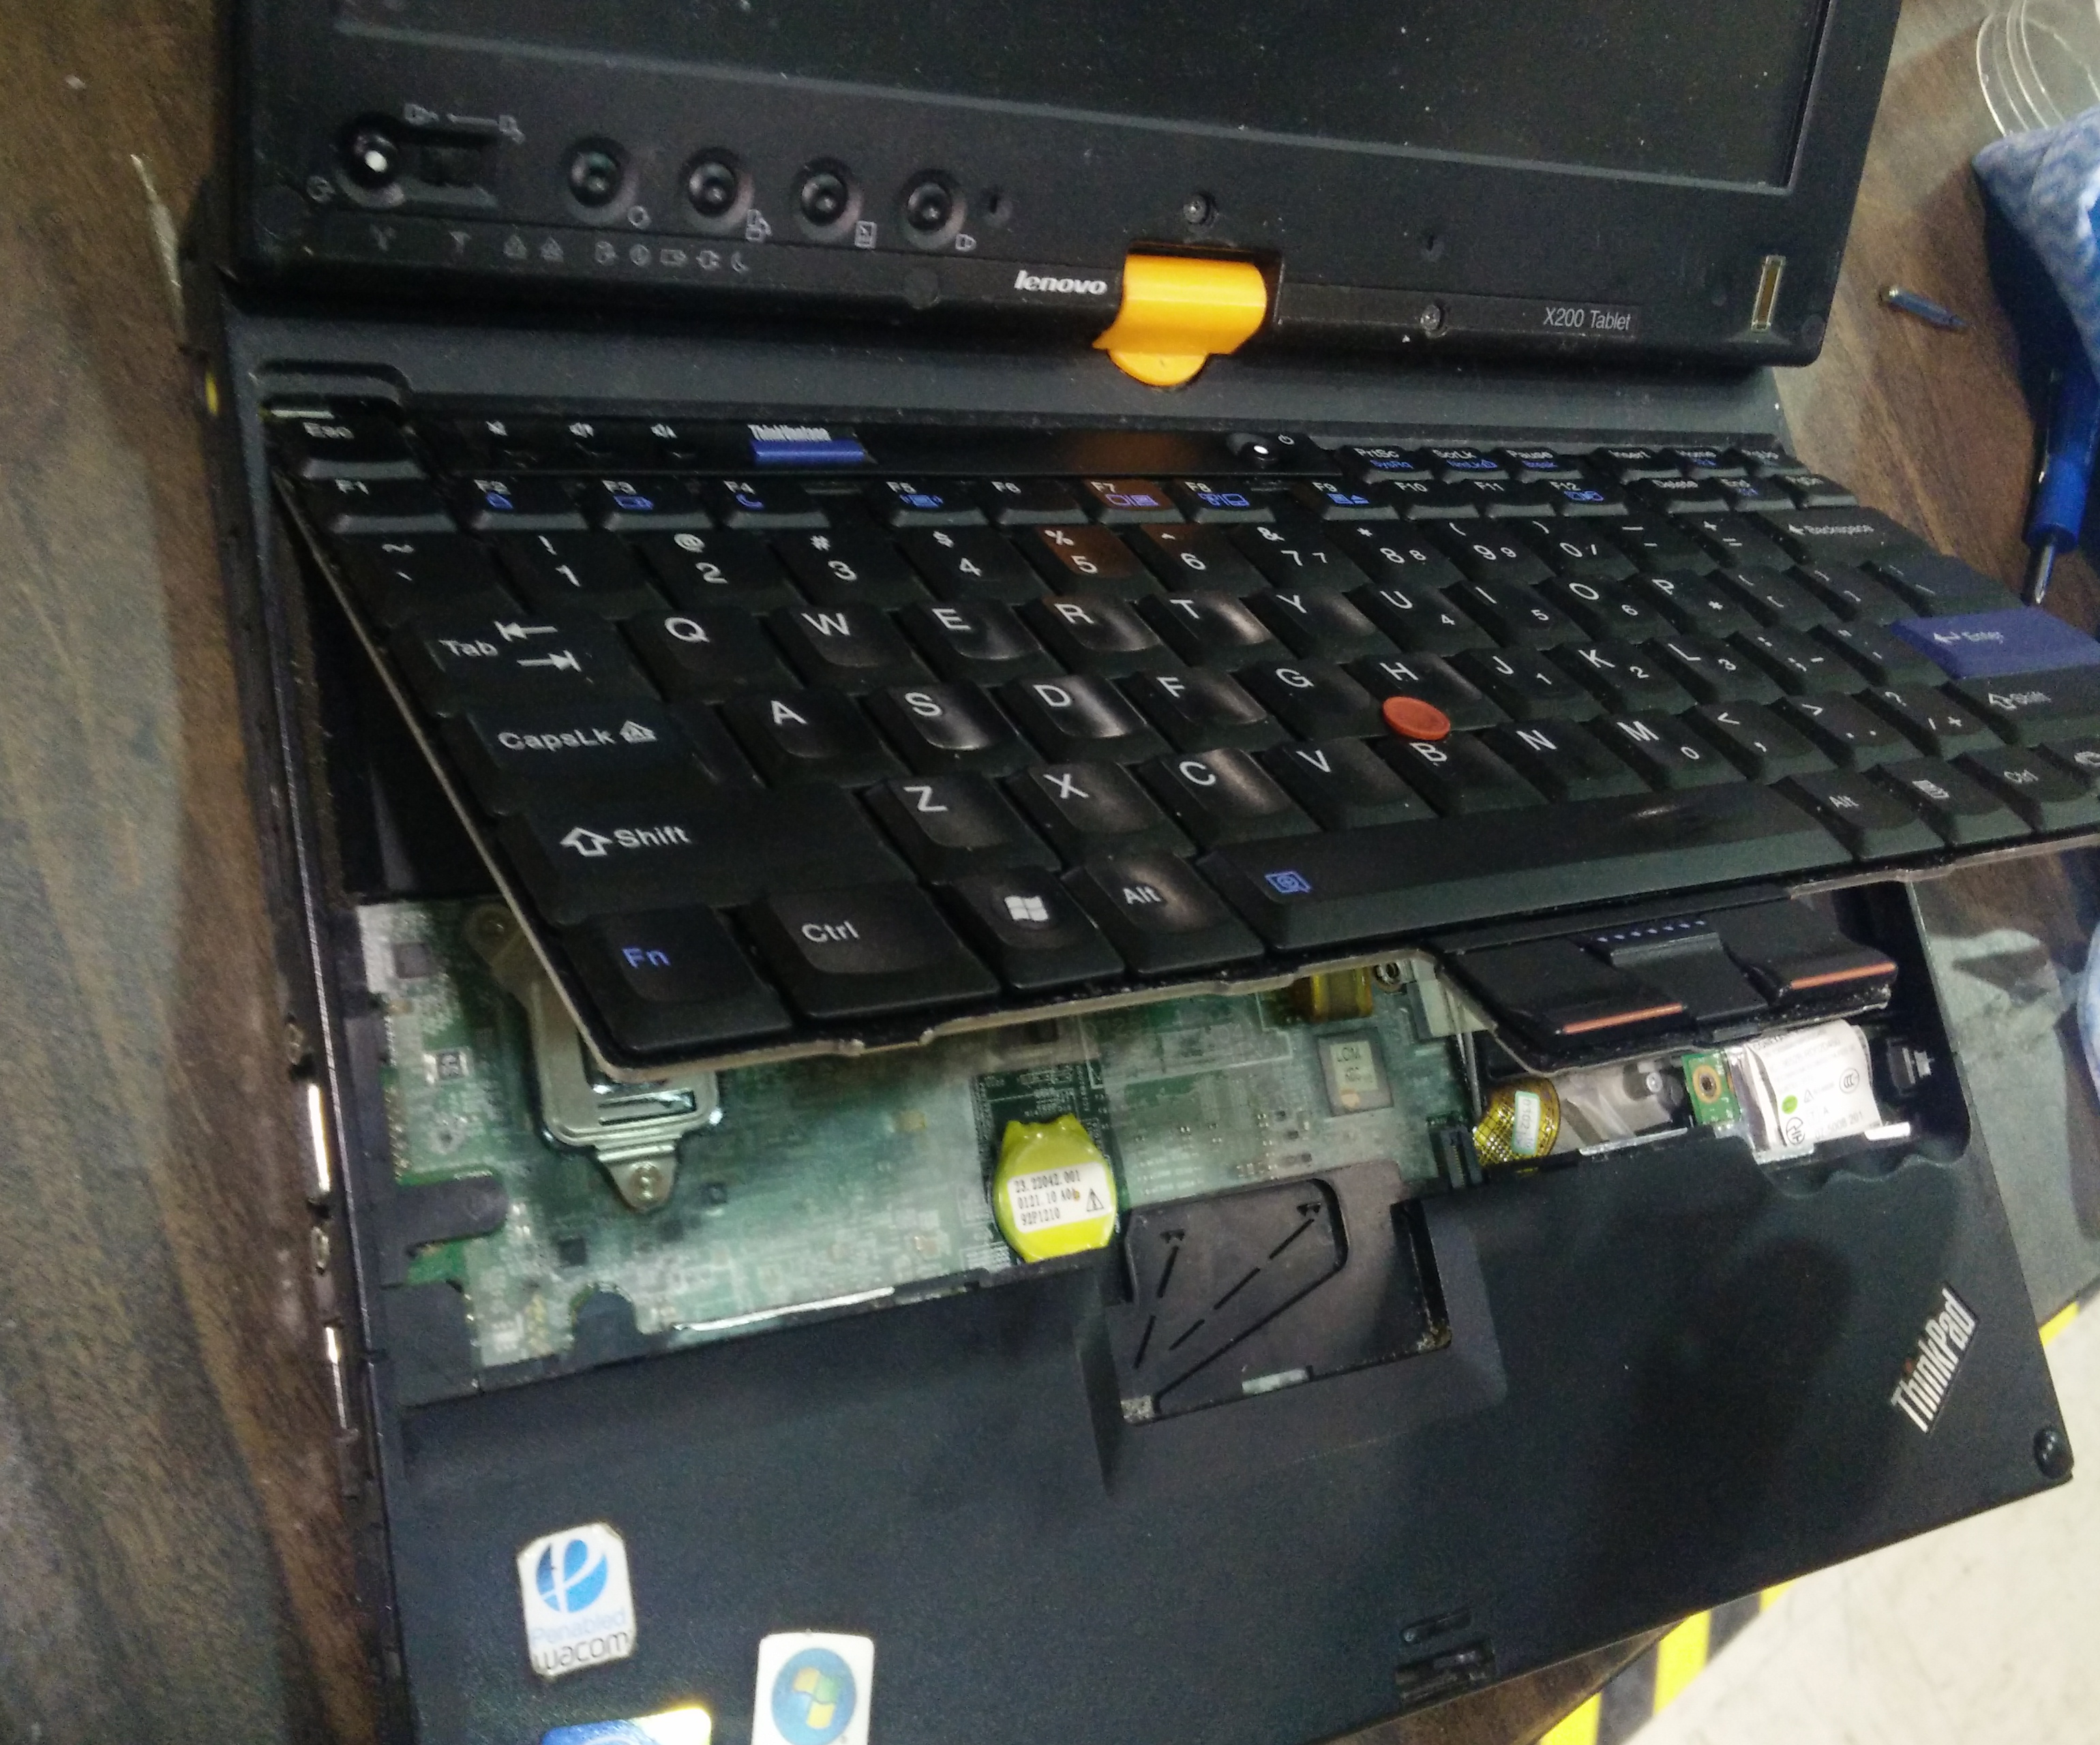
\includegraphics[width=0.5\textwidth]{insertkeyboard.jpg}
		\caption{The keyboard being inserted into the frame}
		\label{fig:angleinsert}
	\end{figure}

	\item Allow the keyboard to lay flat in the housing, applying gentle pressure if necessary.
	\item Put pressure on the keyboard and slide it away the screen until the retaining tabs near the bottom of the keyboard are under the palm rest.
	\begin{figure}[H]
		\centering
		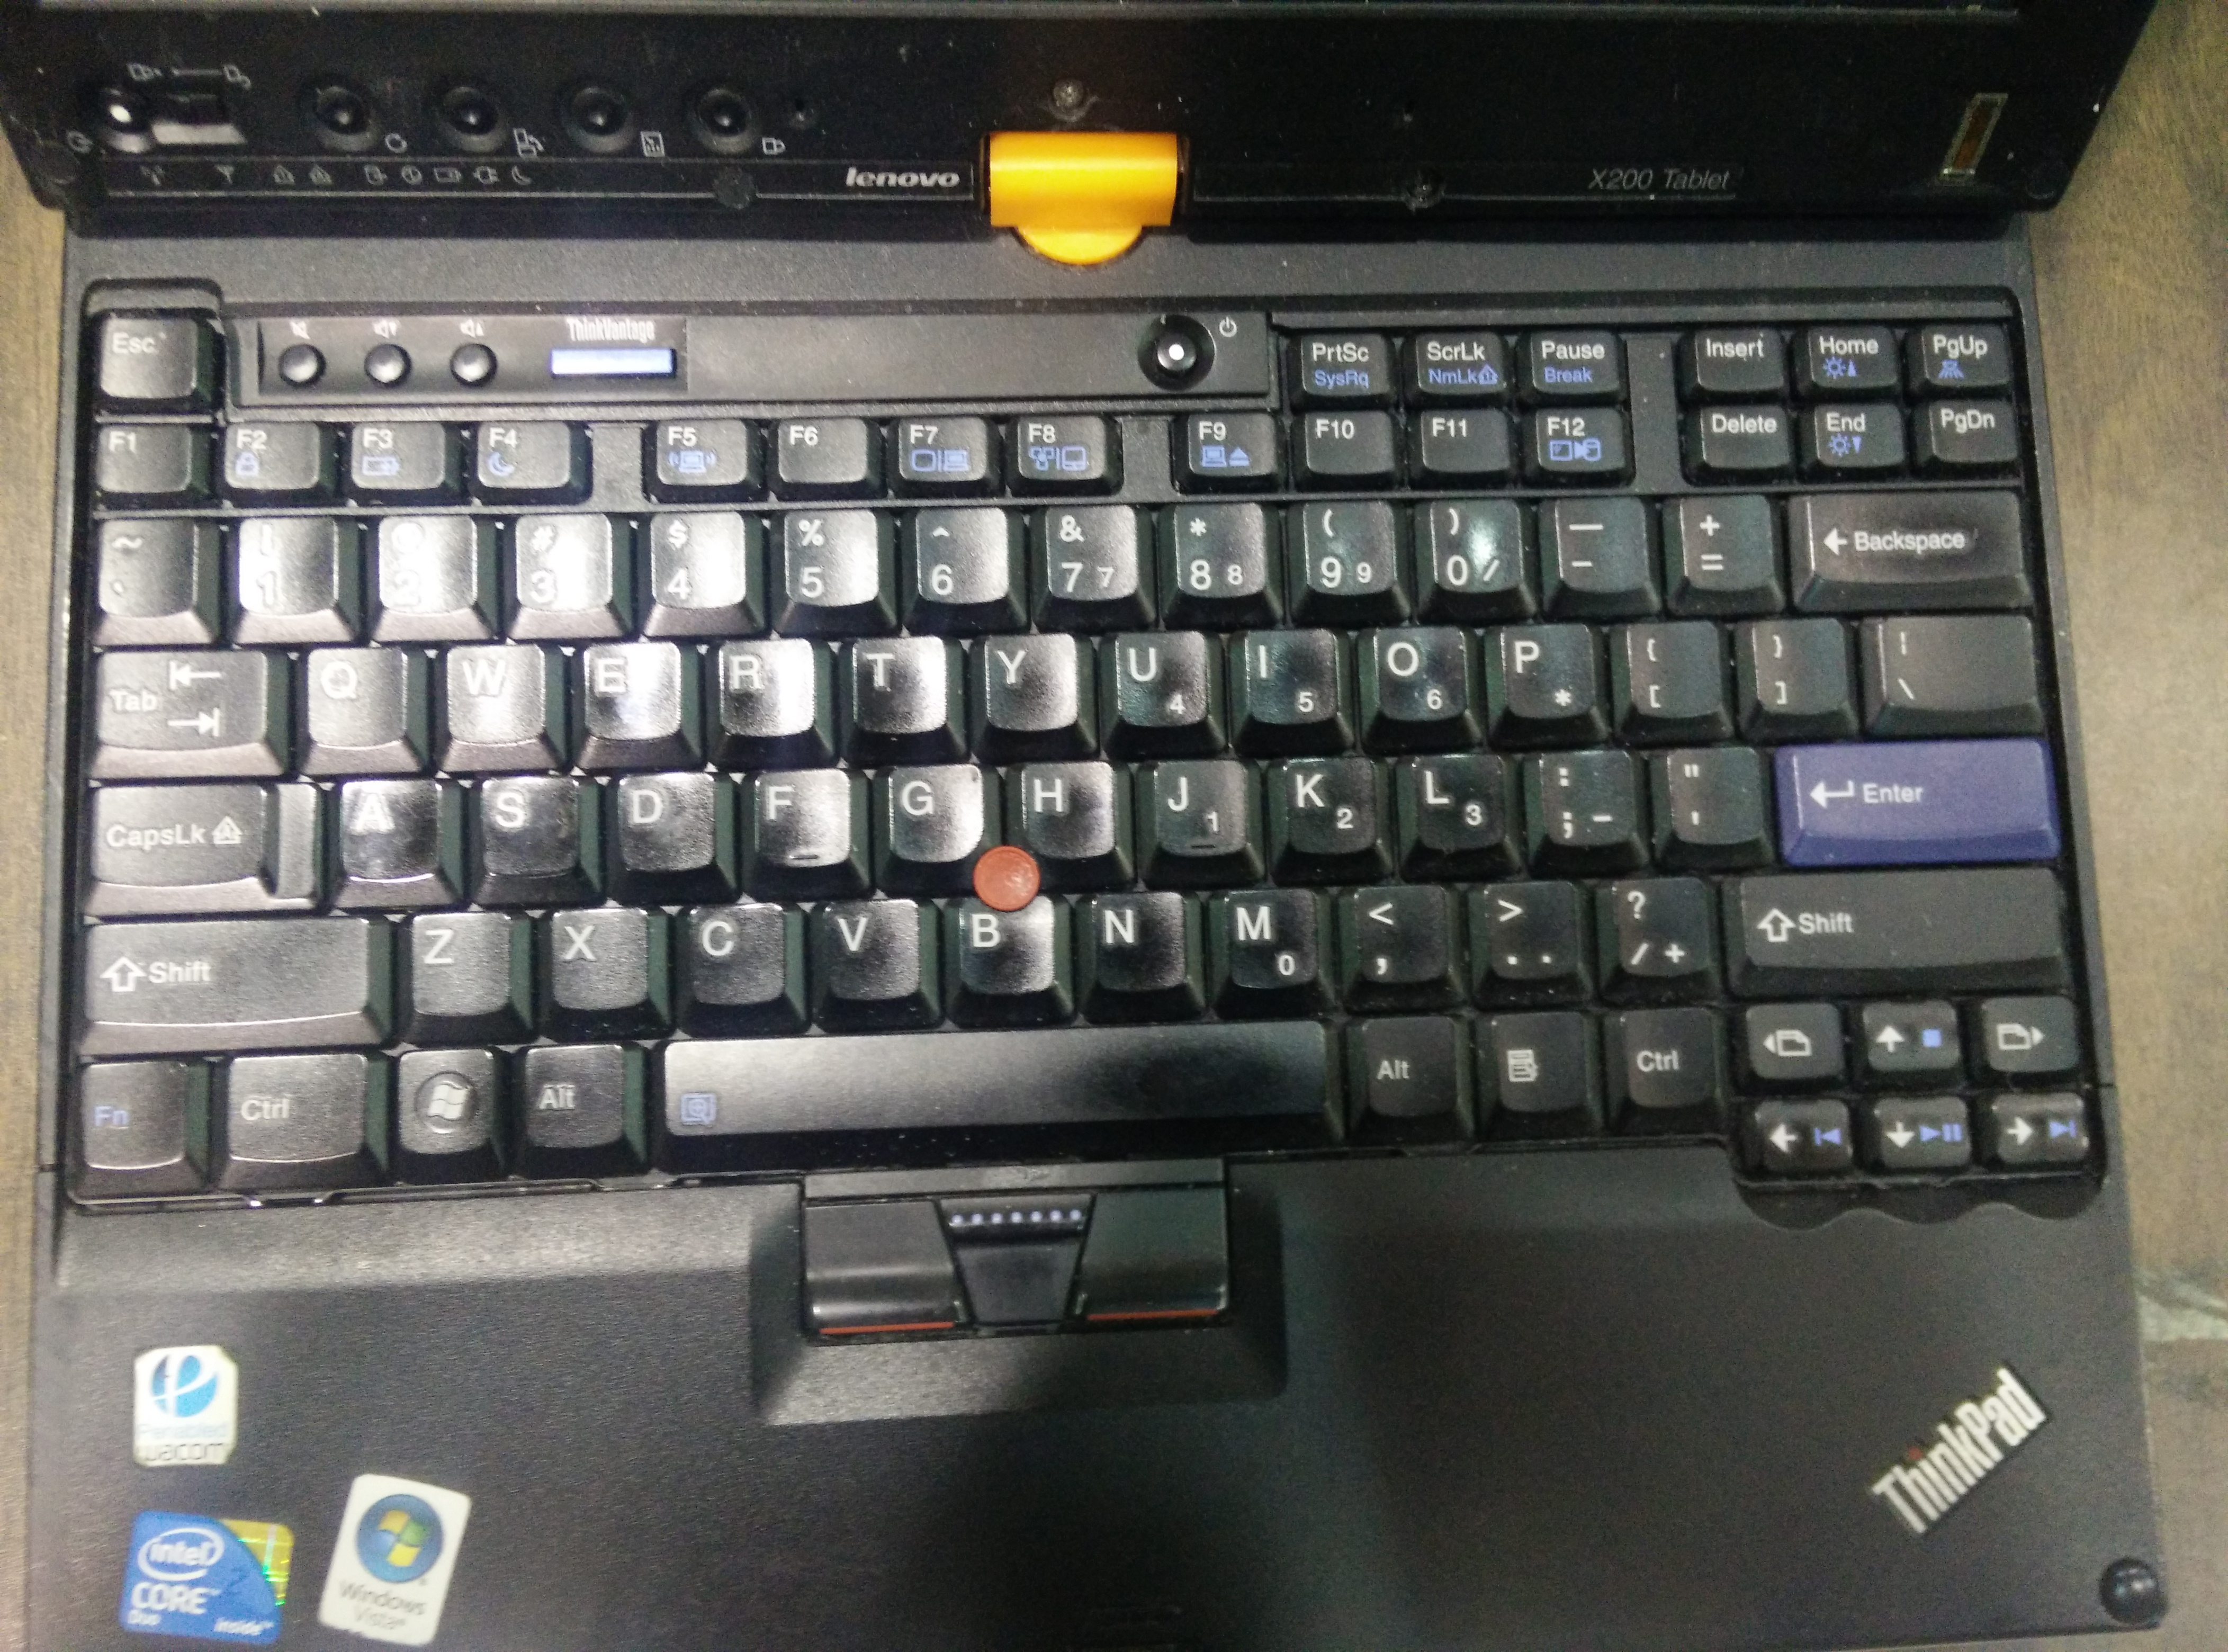
\includegraphics[width=0.5\textwidth]{keyboardlayflat.jpg}
		\caption{The keyboard laying flat in the housing.}
	\end{figure}

	\item Replace the four black screws from the bottom of the laptop. (Refer to Figure \ref{fig:screws} if necessary)

\end{enumerate}

\section*{Conclusion}
You have now successfully cleaned the keyboard on your ThinkPad X200T.
For information on how to replace and/or clean other parts of your laptop, please refer to the \textit{Thinkpad X200 Tablet and X201 Tablet Hardware Maintenance Manual} available at \url{https://github.com/Gigahawk/mech226flowchart/blob/master/docs/maintenancemanual.pdf}

\end{document}
